%!TEX program = xelatex

% safe参数解决与\!在内的多个冲突
% \sups命令可能被重定义,xeCJK放在tipa后
\RequirePackage[safe]{tipa}
\documentclass[a4paper, zihao=-4, linespread=1]{ctexrep}
  \xeCJKsetup{CJKmath=true}
  \renewcommand{\CTEXthechapter}{\thechapter}


% 中文支持
% \iffalse与\fi可以实现“多行注释”
\iffalse
\usepackage[slantfont,boldfont]{xeCJK}
	\setCJKmainfont[BoldFont=SimHei,ItalicFont=KaiTi]{SimSun}
	\setCJKmathfont{STXinwei}
\usepackage{indentfirst}
\fi
\setCJKmathfont{KaiTi}
\newCJKfontfamily[zhxinwei]\xinwei{STXinwei}

% 数学环境
\usepackage{amsmath}
  \newcommand{\ue}{\mathrm{e}}
  \newcommand{\ud}{\mathop{}\negthinspace\mathrm{d}}
\usepackage{amssymb}
\usepackage{mathrsfs} % 线性代数字体
    % overline的替代命令
\newcommand{\closure}[2][3]{{}\mkern#1mu\overline{\mkern-#1mu#2}}
\usepackage{yhmath} % 左下-右上省略号
\usepackage{mathtools} % dcases环境
\usepackage{amsthm} % 定理环境
  \theoremstyle{definition}\newtheorem{laws}{Law}[section]
  \theoremstyle{plain}\newtheorem{ju}[laws]{Jury}
  \theoremstyle{remark}\newtheorem*{marg}{Margaret}
\usepackage{esint} % 多重积分,需放在amsmath后

% 下划线宏包
\usepackage{ulem}
% LaTeX符号宏包
\usepackage{hologo}
	\newcommand{\xelatex}{\Hologo{XeLaTeX}}
	\newcommand{\bibtex}{\Hologo{BibTeX}}
% 其他符号
\usepackage{wasysym}
% 带箱小页
\usepackage{boxedminipage}
% 绘图
\usepackage{tikz}
	\usetikzlibrary{calc}
	\newcommand{\tikzline}[1]{{#1\tikz{\draw[#1,line width=9](0,0)--(0.5,0);}}, }

% 奇怪的小定义
\newcommand{\dpar}{\\ \mbox{}}	% 空两行
\newcommand{\qd}[1]{{\bfseries{#1}}}	% 强调
\newcommand{\co}[1]{{\bfseries{#1}}}   % Style of concept
\newcommand{\RED}[1]{{\color{cyan}{#1}}}
\newcommand{\cmmd}[1]{\fbox{\texttt{\char92{}#1}}}
\newcommand{\charef}[1]{第\ref{#1}章}
\newcommand{\secref}[1]{第\ref{#1}节}
\newcommand{\pref}[1]{第\pageref{#1}页}
\newcommand{\fref}[1]{图\ref{#1}}
\newcommand{\tref}[1]{表\ref{#1}}

% 编号列表宏包,并自定义了三个列表
\usepackage[inline]{enumitem}
	\setlist[enumerate]{label=\arabic* - ,font=\bfseries,itemsep=0pt}
	\setlist[itemize]{label=$\bullet$,font=\bfseries,leftmargin=\parindent}
	\setlist[description]{font=\bfseries\uline}

\newenvironment{fead}{\setlength{\parskip}{0pt}
	\begin{description}[font=\bfseries\uline,labelindent=\parindent]
		\setlength{\itemsep}{0pt}\setlength{\parsep}{0pt}\setlength{\parskip}{0pt}}
	{\end{description}}
% 带宽度的
\newenvironment{para}{\setlength{\parskip}{0pt}
	\begin{description}[font=\bfseries\ttfamily]
		\setlength{\itemsep}{0pt}\setlength{\parsep}{0pt}\setlength{\parskip}{0pt}}
	{\end{description}}
\newenvironment{feae}{\setlength{\parskip}{0pt}
	\begin{enumerate}[font=\bfseries,labelindent=0pt]}
	{\end{enumerate}}
\newenvironment{feai}{\setlength{\parskip}{0pt}
	\begin{itemize}[font=\bfseries]
		\setlength{\itemsep}{0pt}\setlength{\parsep}{0pt}\setlength{\parskip}{0pt}}
	{\end{itemize}}
\newenvironment{inlinee}
{\begin{enumerate*}[label=(\arabic*), font=\rmfamily, before=\unskip{:},itemjoin={{;}},itemjoin*={{,以及:}}]}
	{\end{enumerate*}。}

% 目录和章节样式
\usepackage{titlesec}
\usepackage{titletoc}   % 用于目录

\titlecontents{chapter}[1.5em]{}{\contentslabel{1.5em}}{\hspace*{-2em}}{\hfill\contentspage}
\titlecontents{section}[3.3em]{}{\contentslabel{1.8em}}
	{\hspace*{-2.3em}}{\titlerule*[8pt]{$\cdot$}\contentspage}
\titlecontents*{subsection}[2.5em]{\small}{\thecontentslabel{} }{}{, \thecontentspage}[;\qquad][.]
% 章节样式
\setcounter{secnumdepth}{3} % 一直到subsubsection
\newcommand{\chaformat}[1]{%
	\parbox[b]{.5\textwidth}{\hfill\bfseries #1}%
	\quad\rule[-12pt]{2pt}{70pt}\quad
	{\fontsize{60}{60}\selectfont\thechapter}}
\titleformat{\chapter}[block]{\hfill\LARGE\sffamily}{}{0pt}{\chaformat}[\vspace{2.5pc}\large
	\startcontents\printcontents{}{1}{\setcounter{tocdepth}{2}\songti}]
%\titleclass{\section}{top}
%\titleformat{\section}{\Large\bfseries}{\thesection}{0.5em}{}
\titleformat*{\section}{\centering\Large\bfseries}
\titleformat{\subsubsection}[hang]{\bfseries\large}{\rule{1.5ex}{1.5ex}}{0.5em}{}
% 扩展章节
\newcommand{\starsec}{\noindent\fbox{\S\textit{注意:本章节是一个扩展阅读章节。}}
	\\ \mbox{}}

\renewcommand{\contentsname}{目录}
	\renewcommand{\tablename}{表}
	\renewcommand\arraystretch{1.2}	% 表格行距
	\renewcommand{\figurename}{图}
% 设置不需要浮动体的表格和图像标题
\setlength{\abovecaptionskip}{5pt}
\setlength{\belowcaptionskip}{3pt}
\makeatletter
\newcommand\figcaption{\def\@captype{figure}\caption}
\newcommand\tabcaption{\def\@captype{table}\caption}
\makeatother
% 图表
\usepackage{array,multirow}
  \setlength\extrarowheight{2pt} % 行高增加
\usepackage{longtable}
\usepackage{graphicx}
  \graphicspath{{./tikz/}}
% 页面修正宏包
\usepackage{geometry}
\geometry{top = 1in}

% 代码环境
\usepackage{listings}
% Avoid copy line numbers of the listing code (Invalid for SumatraPDF Reader)
\usepackage{accsupp}
	\newcommand{\emptyaccsupp}[1]{\BeginAccSupp{ActualText={}}#1\EndAccSupp{}}
% Color
\usepackage{xcolor}
  \newcommand{\scol}[1]{\colorbox{#1}{\rule{0em}{1ex}}\,#1}
	\definecolor{commentcolor}{RGB}{85,139,78}
	\definecolor{numbercolor}{RGB}{166,206,168}
	\definecolor{stringcolor}{RGB}{206,145,108}
	\definecolor{keywordcolor}{RGB}{34,34,250}
	\definecolor{backcolor}{RGB}{220,220,220}
	\definecolor{packagecolor}{RGB}{0,128,0}
	\definecolor{envicolor}{RGB}{185,70,15}
% LaTeX Code Style
\lstset{language=[LaTeX]TeX,
		basicstyle=\small\ttfamily,
		commentstyle=\color{commentcolor},
		keywordstyle=\color{keywordcolor},
		stringstyle=\color{stringcolor},
		showstringspaces=false,
		% Package/Tikz-Lib Using
		classoffset=0,
		morekeywords={begin,end,usetikzlibrary},
		keywordstyle=\color{keywordcolor},
		classoffset=1,
		morekeywords={article,report,book,
			xeCJK,tikz,
			calc},
		keywordstyle=\color{packagecolor},
		classoffset=2,
		morekeywords={document,tikzpicture},
		keywordstyle=\color{envicolor},
		% Line Number Style
		numbers=left,
		numberstyle=\tiny\emptyaccsupp,
		stepnumber=1,
		% Frame and Background Color
		frame=single,
		framerule=0pt,
		backgroundcolor=\color{backcolor},
		% Spaces
		% belowskip=\medskipamount,
		emptylines=1,
		escapeinside=``}

\lstnewenvironment{latex}[1]{\lstset{#1}}{}
\newcommand{\latexline}[1]{{\lstinline[language=TeX,basicstyle=\small\ttfamily]{#1}}}

% Tikz Code
\lstdefinelanguage{tikzlang}{
	classoffset=0, % 蓝色的keyword
	morekeywords={begin,end,newcommand,
		draw,node,coordinate,tikzstyle,foreach},
	keywordstyle=\color{keywordcolor},
	classoffset=1, % 棕色的其他关键字
	morekeywords={tikzpicture,grid,at,
		thick,thin,very,ultra,
		red,green,yellow,blue,cyan,magenta,black,
		    gray,darkgray,lightgray,brown,lime,
		    olive,orange,pink,purple,teal,violet,white},
	keywordstyle=\color{envicolor},
	morecomment=[l]{\%},
	morecomment=[s]{/*}{*/},
	morestring=[b]',
	% Escape
	escapeinside=``
}
\lstnewenvironment{tikzcode}[1]{\lstset{language=tikzlang,basicstyle=\small\ttfamily,
		breaklines=true,%backgroundcolor=\color{white},
		linewidth=0.7\linewidth,#1}}{}

% 附录
\usepackage{appendix}
\renewcommand{\appendixname}{App.}

% 行号
\usepackage{lineno}

% 代码输入环境
\usepackage{verbatim,xcolor}
\newbox\savedlines
\newtoks\savedtokens
\makeatletter
\def\codeshow{%
\global\savedtokens={}%
\def\verbatim@processline{%
{\setbox0=\hbox{\the\verbatim@line}%
\hsize=\wd0
\the\verbatim@line\par}%
\global\savedtokens=\expandafter{\the\expandafter\savedtokens\the\verbatim@line^^J}}%
\@tempswatrue
\setbox0=\vbox\bgroup\parskip=0pt\topsep=0pt\partopsep=0pt
\verbatim}
\def\endcodeshow{\endverbatim%
\unskip\setbox0=\lastbox\egroup
\global\setbox\savedlines=\box0
\addvspace{1em}\par\noindent%
\colorbox{lightgray}{%
\begin{minipage}{.55\textwidth}{\usebox\savedlines}\end{minipage}}%
\hfill\fbox{\parbox{.40\textwidth}%
{\scantokens\expandafter{\the\savedtokens\unskip\endinput}}}%
\par\addvspace{1em}}
\makeatother

\usepackage{booktabs}

\bibliographystyle{plain}
\renewcommand{\bibname}{参考文献}
\usepackage[square,super,sort&compress]{natbib}

% 引用
\usepackage{hyperref}
\hypersetup{colorlinks, bookmarksopen = true, bookmarksnumbered = true, pdftitle=LaTeX-cn, pdfauthor=K.L Wu, pdfstartview=FitH}

\title{简单粗暴\LaTeX }
\author{K.L Wu\\
  {\kaishu 本手册是\href{https://github.com/wklchris/Note-by-LaTeX}{wklchris-GitHub}的\LaTeX{}-cn项目}
}
\date{第一版已定稿。\\
  最后更新于:\today}

\begin{document}

\maketitle

\tableofcontents

\chapter{序}

\noindent{\Huge\xinwei 第一稿序}\dpar\dpar

其实在之前我是有一稿手册的,开始撰写的日期大概在2015年4月。但是自己觉得写得太烂,因此索性推倒重写了这一版。这一版的主要特征是:
\begin{feae}
  \item 我希望能够吸引初学者快速上手,解决手头的问题。因此去掉了枯燥的讲解和无穷无尽的宏包用法介绍,直接使用实例;
  \item 力求突出实用性。当然,也会提点一些可以深入学习的内容,读者可以自行查阅,或者阅读本手册中的扩展阅读章节(即带星号*的章节)。
  \item 本手册使用的编辑器为\TeX Studio,而非之前的商业软件WinEdt. 这使得学习\LaTeX 的门槛更低。当然了,你有权使用任何编辑器。
\end{feae}

手册一共分为五大部分\cite{LHY2013latex,lamport1986document,mittelbach2004latex,partl2016}:
\begin{fead}
\item[基础] 包括标点、缩进、距离、章节、字体、颜色、注释、引用、封面、目录、列表、图表、页面等详细内容。
\item[数学排版] 包括数学符号、公式、编号等内容。
\item[进阶] 主要是自定义命令,帮助你更高效、更简洁地书写你的文档。
\item[Tikz绘图*] 附加章节,需要读者取消注释后重编译。
\item[附录] 帮助你快速查找一些你想要的东西。
\end{fead}

由于工作全部由我一人完成,限于视野,难免存在错漏之处。恳请读者指正。有任何使用中遇到的手册中无法解决的问题,欢迎向我提出。另外,我推荐\emph{The \LaTeX{} Companion}, 一个优秀的知识补漏手册。

最后,还要感谢在\LaTeX 学习中为我解答疑惑的同学,特别是来自\LaTeX 度吧的吧友;本手册中许多的解决方案都是由他们提供的。我谨在此记录。

\vfill

\begin{flushright}
Mail: wklchris@hotmail.com\dpar

Chris Wu

September 17, 2016 于Davis, CA
\end{flushright}



\chapter{\LaTeX{}基础}
\section{第一份文稿}

编辑器的配置大概是需要讲解一下的,毕竟对于初学者来说是很头疼的事情。本手册就以\TeX Studio为例进行配置。首先你应该安装一个\TeX{} Live,它是完全免费的,网址:\url{http://tug.org/texlive/}.

虽然它体积较大,但是却是最一劳永逸、最不需要花时间取配置的方法,同时它大概也是功能支持最强的\LaTeX 发行版。

打开\TeX Studio后,选择选项$\rightarrow$ 设置\TeX Studio $\rightarrow$ 构建$\rightarrow$ 默认编译器,选择\xelatex{}. 这主要是基于中文文档编译的考虑,同时\xelatex 也能很好地编译英文文档。我建议始终使用它作为默认编译器。\dpar

之后你可以在编译窗口输入一篇小文档,并保存为tex文件进行测试:
\begin{latex}{}
\documentclass{ctexart}
\begin{document}
  Hello, world!
  你好,世界!
\end{document}
\end{latex}

点击编译按钮生成,F7查看。生成的pdf在你的tex文件保存目录中。具体各行的含义我们会在后文介绍。

\section{认识\LaTeX}
\subsection{命令与环境}
\LaTeX 中的\co{命令}通常是由一个反斜杠加上命令名称,再加上花括号内的参数构成的。比如:
\begin{latex}{}
\documentclass{ctexart}
\end{latex}

如果有一些选项是备选的,那么通常会在花括号前用方括号标出。比如:
\begin{latex}{}
\documentclass[a4paper]{ctexart}
\end{latex}

在\LaTeX 中,还有一种重要指令叫做\co{环境}。它定义某区段的内容受到环境(即其本身)的控制,区段从\latexline{\\begin{environment}}开始,到\latexline{\\end{environment}}结束的。比如:
\begin{latex}{}
\begin{document}
	...内容...
\end{document}
\end{latex}

同样的,环境也可以使用备选选项,只需要写在begin的后面就行了。

注意:不带花括号的命令后面如果想打印空格,请加上\RED{一对内部为空的花括号}再键入空格。否则空格会被忽略。例如:\verb+\LaTeX{} Studio+.

\subsection{保留字符}

\LaTeX 中有许多字符有着特殊的含义,在你生成文档时不会直接打印。例如每个命令的第一个字符:反斜杠。单独输入一个反斜杠在你的行文中不会有任何帮助,甚至可能产生错误。\LaTeX 中的保留字符有:
\begin{center}
\texttt{\# \$ \% \^ \& \_ \{ \} \char92}
\end{center}

它们的作用分别是:
\begin{para}
\item[\#{}:] 自定义命令时,用于标明参数序号。
\item[\${}:] 数学环境命令符。
\item[\%{}:] 注释符。在其后的该行命令都会视为注释。如果在回车前输入这个命令,可以防止行末\LaTeX 插入一些奇怪的空白符。
\item[\^{}:] 数学环境中的上标命令符。
\item[\&{}:] 表格环境中的跳列符。
\item[\_{}:] 数学环境中的下标命令符。
\item[\{and\}:] 花括号用于标记命令的必选参数,或者标记某一部分命令成为一个整体。
\item[\char92{}:] 反斜杠用于开始各种\LaTeX 命令。
\end{para}

以上除了反斜杠外,均能用前加反斜杠的形式输出。即你只需要键入:
\begin{center}
\verb|\# \$ \% \^ \& \_ \{ \}|
\end{center}

唯独反斜杠的输出比较头痛,你可以尝试:
\begin{verbatim}
$\backslash$
\textbackslash
\texttt{\char92}
\end{verbatim}

另外需要说明的是,波浪线{\texttt{\~}}用来输出一个禁止在该处断行的空格,不能够直接输出。你可以通过命令\verb+$\sim$+,\verb|\~|或者仿上换成char126来产生一个。你也可以尝试命令\latexline{\\textasciitilde}。

\subsection{导言区}
任何一份\LaTeX{}文档都应当包含以下结构:
\begin{latex}{}
\documentclass[`\itshape options`]{doc-class}
\begin{document}
    ...
\end{document}
\end{latex}

其中,在语句\latexline{\\begin{document}}之前的内容称为\co{导言区}。导言区可以留空,以可以进行一些文档的准备操作。你可以粗浅地理解为:\RED{导言区即模板定义}。\dpar

文档类的参数doc-class和可选选项{\textit{options}}有以下取值:
\begin{table}[!htb]
\begin{center}
	\caption{文档类和选项}
	\label{tb:documentclass}
	\begin{tabular}{p{5em} @{\ -\ } p{24em}}
		\hline
		\multicolumn{2}{l}{\bfseries doc-class文档类} \\
		\hline
		article   & 科学期刊,演示文稿,短报告,邀请函。\\
		proc      & 基于article的会议论文集。\\
		report    & 多章节的长报告、博士论文、短篇书。\\
		book      & 书籍。\\
		slides    & 幻灯片,使用了大号Scans Serif字体。\\
		\hline
		\multicolumn{2}{l}{\bfseries\itshape options} \\
		\hline
		字体     & 默认10pt,可选11pt和12pt.\\
		页面方向 & 默认竖向portrait,可选横向landscape。\\
		纸张尺寸 & 默认letterpaper,可选用a4paper, b5paper等。\\
		分栏     & 默认onecolumn,还有twocolumn。\\
		双面打印 & 有oneside/twoside两个选项,用于排版奇偶页。article/report默认单面。\\
		章节分页 & 有openright/openany两个选项,决定是在奇数页开启新页或是任意页开启新页。注意article是没有chapter(``章'')命令的,默认任意页。\\
		公式对齐 & 默认居中,可改为左对齐fleqn;默认编号居右,可改为左对齐leqno。\\
		\hline
	\end{tabular}
\end{center}
\end{table}

在本文中,多数的文档类提及的均为report/book类。如果有article类将会特别指明。其余的文档类不予说明。本手册排版即使用了book类。\dpar

在导言区最常见的是\co{宏包}的加载工作,命令形如:\latexline{\\usepackage{package}}。通俗地讲,宏包是指一系列已经制作好的功能``模块'',在你需要使用一些原生\LaTeX 不带有的功能时,只需要调用这些宏包就可以了。比如本文的代码就是利用{\texttt{listings}}宏包实现的。

宏包的具体使用将参在各部分内容说明中进行讲解。如果你想学习一个宏包的使用,按Win+R组合键呼出运行对话框,输入texdoc加上宏包名称即可打开宏包帮助pdf文档。例如:\verb|texdoc xeCJK|

\subsection{错误的排查}
\label{subsec:debug}
在编辑器界面上,下方的日志是显示编译过程的地方。在你编译通过后,会出现这样的字样:
\begin{feai}
	\item {\qd{Errors错误}}:严重的错误。一般地,编译若通过了,该项是零。
	\item {\qd{Warnings警告}}:一些不影响生成文档的瑕疵。
	\item {\qd{Bad Boxes坏箱}\footnote{Box是\LaTeX{}中的一个特殊概念,具体将在\hyperref[sec:box]{这里}进行讲解。}}:指排版中出现的长度问题,比如长度超出(Overfull)等。后面的Badness表示错误的严重程度,程度越高数值越大。这类问题需要检查,排除Badness高的选项。
\end{feai}

你可以向上翻阅控制台记录,来找到Warning开头的记录,或者Overfull/ Underfull开头的记录。这些记录会指出你的问题出在哪一行(比如line 1-2) 或者在输出pdf的哪一页(比如active [12]。注意,这个12表示页面显示页码或者计数器计数页码,而不是文件打印出来的真实页码)。此外你可以还需要了解:
\begin{feai}
	\item 值得指出的是,由于\LaTeX{}的编译原理(第一次生成aux文件,第二次再引用它),目录想要合理显示\qd{需要连续编译两次}。在连续编译两次后,你会发现一些Warnings会在第二次编译后消失。在\TeX Studio中,你可以只单击一次“构建并查看”,它会检测到文章的变化并自动决定是否需要编译两次。
	\item 对于大型文档,寻找行号十分痛苦。你需要学会合理地拆分tex文件,参阅\secref{sec:include}的内容。
\end{feai}

这里也推荐宏包\texttt{syntonly},在导言区加入它支持的\latexline{\\syntaxonly}命令,会只排查语法错误而不生成任何文档,这可以使你更快地编译。不过它似乎不太稳定,例如本文档可以正常编译,但是使用该命令时则会出错。

\subsection{文件输出}
\LaTeX{}的输出一般推荐pdf格式,由\LaTeX 直接生成dvi的方法并不推荐。

你在tex文档的文件夹下可能看到的其他文件类型:
\begin{tabbing}
	.sty{\hspace{2em}}\=宏包文件\\
	.aux    \> 用于储存交叉引用信息的文件。因此,在更新交叉引用(公式编号、\\
	\> 大纲级别)后,需要编译两次才能正常显示。\\
	.log    \> 记录上次编译的信息。\\
	.toc    \> 目录文件。\\
	.idx    \> 如果文档中包含索引,该文件用于储存索引信息。\\
	.lof    \> 图形目录。\\
	.lot    \> 表格目录。
\end{tabbing}

有时\LaTeX 的编译出现异常,你需要删除文件夹下除了tex以外的文件再编译。此外,在某些独占程序打开了以上的文件时(比如用Acrobat打开了pdf),编译可能出现错误。请在编译时确保关闭这些独占程序。

\section{标点与强调}
\subsection{引号}
单引号并不使用两个\verb|'|符号组合。左单引号是重音符\verb|`|(键盘上数字1左侧),而右单引号是常用的引号符。英文中,\RED{左双引号就是连续两个重音符}。

英文下的引号嵌套需要借助\verb|\thinspace|命令分隔,比如:

\begin{codeshow}
``\thinspace`Max' is here.''
\end{codeshow}

中文下的单引号和双引号你可以用中文输入法直接输入。

\subsection{破折、省略号与短横}
英文的短横分为三种:
\begin{feai}
\item 连字符:输入一个短横:\verb|-|,效果如daughter-in-law
\item 数字起止符:输入两个短横:\verb|--|,效果如:page 1--2
\item 破折号:输入三个短横:\verb|---|,效果如:Listen---I'm serious.
\end{feai}

中文的破折号你也许可以直接使用日常的输入方式。中文的省略号同样。但是注意,\RED{英文的省略号使用\latexline{\\ldots}这个命令而不是三个句点}。

至于减号,也许你应该借助于数学环境来输入:\verb|$-$|.

\subsection{强调:粗与斜}
\LaTeX 中专门有个叫做\latexline{\\emph{text}}的命令,可以强调文本。对于通常的西文文本,上述命令的作用就是斜体。如果你对一段已经这样转换为斜体的文本再使用这个命令,它就会取消斜体,而成为正体。

西文中一般采用上述的斜体强调方式而不是粗体,例如在说明书名的时候就会使用以上命令。关于字体的更多内容参考\hyperref[sec:font]{字体}这一节。

\subsection{下划线与删除线}
\LaTeX 原生提供了\latexline{\\underline}命令简直烂的可以,建议你使用ulem宏包下的\texttt{uline}命令代替。ulem宏包还提供了一系列有用的命令:

\begin{codeshow}
\uline{下划线} \\
\uuline{双下划线} \\
\dashuline{虚下划线} \\
\dotuline{点下划线} \\
\uwave{波浪线} \\
\sout{删除线} \\
\xout{斜删除线}
\end{codeshow}

需要注意的是,ulem宏包重定义了\verb|\emph|命令,\RED{使得原来的加斜强调变成了下划线、原来的两次强调就取消强调变成了两次强调就双下划线},同时也支持换行文本。

\subsection{其他}
角度符号或者温度符号需要借助数学模式\verb|$...$|输入:

\begin{codeshow}
$30\,^{\circ}$三角形 \\
$37\,^{\circ}\mathrm{C}$
\end{codeshow}

然后是欧元符号,可能需要用到textcomp宏包,然后调用\latexline{\\texteuro}命令就可以了。

其次是千位分隔符,比如\verb|1\,000\,000|。如果你不想它在中间断行就在外侧再加上一个\latexline{\\mbox}命令。

再次是注音符号,比如\^o,也常用于拼音声调,参考\hyperref[app:phonetic]{注音符号表}部分的附录内容。如果你想输入音标,请使用tipa宏包\footnote{tipa会重定义\texttt{\char92{}!}命令,因此请使用\texttt{\negthinspace}代替,或在加载时使用safe选项。},同样参考附录A。

最后,介绍hologo宏包,它可以输出许多\TeX 家族标志。其实\LaTeX 原生自带了\latexline{\\LaTeX \TeX}等命令。而hologo宏包支持的命令是:

\begin{codeshow}
% 大写H表示符号的首字母也大写
\hologo{XeLaTeX} \Hologo{BibTeX}
\end{codeshow}

\section{格式控制}
首先了解一下\hologo{LaTeX}的长度单位:
\begin{fead}
  \item[pt] point,磅。\label{sec:length}
  \item[pc] pica。1pc=12pt,四号字大小
  \item[in] inch,英寸。1in=72.27pt
  \item[bp] bigpoint,大点。1bp=$\frac{1}{72}$in
  \item[cm] centimeter,厘米。1cm=$\frac{1}{2.54}$in
  \item[mm] millimeter,毫米。1mm=$\frac{1}{10}$cm
  \item[sp] scaled point。\Hologo{TeX} 的基本长度单位,1sp=$\frac{1}{65536}$pt
  \item[em] 当前字号下,大写字母M的宽度。
  \item[ex] 当前字号下,小写字母x的高度。
\end{fead}

然后是几个常用的长度宏,更多的长度宏使用会在表格、分栏等章节提到。

\begin{center}
\begin{tabular}{|ll|}
\hline
\textbackslash{}textwidth & 页面上文字的总宽度,即页宽减去两侧边距。\\
\textbackslash{}linewidth & 当前行允许的行宽。\\
\hline
\end{tabular}
\end{center}

有时候你可以使用可变长度,比如“\texttt{5pt plus 3pt minus 2pt}”,表示一个能收缩到3pt也能伸长到8pt的长度。直接使用倍数也是允许的,例如:\latexline{1.5\\parindent}等。

我们通常使用\latexline{\\hspace{len}}和\latexline{\\vspace{len}}这两个命令控制特殊的空格,具体的使用方法参考\hyperref[sec:hvspace]{水平和竖直距离}这一节。

\subsection{空格、换行与分段}
在\LaTeX 中,多个空格会被视为一个,多个换行也会被视为一个。如果你想要禁止\LaTeX 在某个空格处的换行,将空格用\texttt{\char126}命令替代即可,比如“\texttt{Fig.\char126 8}”。

通常的换行方法非常简单:\hologo{LaTeX}会自动转行,然后在每一段的末尾,只需要输入两个回车即可完成分段。如果需要一个空白段落(实质是一个空白行),先输入两个回车,再输入\latexline{\\mbox{}},最后再输入两个回车即可。

在下划线一节的例子中已经给出了强制换行的方式,即两个反斜:\verb|\\|. 不过这样做的缺点在于下一行段首缩进会消失。你可以用\verb|\par|来解决这个问题。

\subsection{分页}
用\latexline{\\newpage}命令开始新的一页。

用\latexline{\\clearpage}命令清空浮动体队列\footnote{参见\hyperref[sec:float]{浮动体}这一节的内容。},并开始新的一页。

用\latexline{\\cleardoublepage}命令清空浮动体队列,并在偶数页上开始新的一页。

注意:以上命令都是基于\verb|\vfill|的。如果要连续新开两页,请在中间加上一个空的箱子(\latexline{\\mbox{}}),如\latexline{\\newpage\\mbox{}\\newpage}。

\subsection{缩进、对齐与行距}
英文的段首不需要缩进。但是对中文而言,段首缩进需要借助indentfirst宏包来完成。你可能还需要使用\latexline{\\setlength{\\indent}{2em}}这样的命令来完成缩进距离的设置。如果在句首强制取消缩进,你可以使用\latexline{\\noindent}命令。

\LaTeX 默认使用两端对齐的排版方式。你也可以使用flushleft, flushright, center这三种环境来构造居左、居中、居右三种效果。特殊的\latexline{\\centering}命令常常用在环境内部(或者一对花括号内部),以实现居中的效果。但请尽量用center环境代替这个老旧的命令。类似的命令还有\latexline{\\raggedleft}来实现居右,\latexline{\\raggedright}来实现居左。更多的空格控制请参考\hyperref[sec:hvspace]{这一节}。

插入制表位、悬挂缩进、行距等复杂的调整参考\hyperref[sec:hvspace]{这部分}的内容。

\section{字体与颜色}
\label{sec:font}
这一节只讨论行文中字体使用。数学环境内字体使用请参考\hyperref[sec:mathfont]{这一节}的内容。

\subsection{字族、字系与字形}
字体(typeface)的概念非常令人恼火,在电子化时代,基本上也都以字体(font)作为替代的称呼。宋体、黑体、楷体,这属于\co{字族};对应到西文就是罗马体、等宽体等。加粗、加斜属于\co{字系和字形}。五号、小四属于\co{字号}。这三者大概可以并称\co{字体}\footnote{本文中的字族、字系等称呼难以找到统一标准,可能并不是准确的名称。}。

\subsection{中西文“斜体”}
首先需要明确一点:\RED{汉字没有加斜体}。平常我们看到的加斜汉字,通常是几何变换得到的结果,非常的粗糙,并不严格满足排版要求;而真正的字形是需要精细的设计的。同时,汉字字体里面也很少有加粗体的设计。

西文一般设有加斜,但是这与“斜体”并不是同一回事。加斜是指某种字族的Italy字系;而斜体,是指Slant字族。在行文中表强调时使用的是前者;在Microsoft Word等软件中看到的倾斜的字母\textit{I},也代表前者。

\subsection{原生字体命令}
\LaTeX 提供了基本的字体命令,包括\tref{tab:fontcommand}中显示的内容。
\begin{table}[!ht]
\centering
\caption{\LaTeX 字体命令表}
\label{tab:fontcommand}
\begin{tabular}{p{3em}<{\centering} @{\ -\quad} >{\ttfamily}l @{\quad-\quad} p{18em}}
\hline
字族 & \char92{}rmfamily & 把字体置为{\rmfamily Roman}罗马字族。\\
     & \char92{}sffamily & 把字体置为{\sffamily Sans Serif}无衬线字族。\\
     & \char92{}ttfamily & 把字体置为{\ttfamily Typewriter}等宽字族。\\
\hline
字系 & \char92{}bfseries & 粗体{\bfseries BoldSeries}字系属性。\\
     & \char92{}mdseries & 中粗体{\mdseries MiddleSeries}字系属性。\\
\hline
字形 & \char92{}upshape  & 竖直{\upshape Upright}字形。 \\
     & \char92{}slshape  & 斜体{\slshape Slant}字形。 \\
     & \char92{}itshape  & 强调体{\itshape Italic}字形。 \\
     & \char92{}scshape  & 小号大写体{\scshape Scap}字形。 \\
\hline
\multicolumn{3}{l}{\ttfamily 如果临时改变字体,使用\char92{}textrm, \char92{}textbf这类命令。}\\
\hline
\end{tabular}
\end{table}

字族、字系、字形三种命令是互相独立的,可以任意组合使用。但这种复合字体的效果有时候无法达到(因为没有对应的设计),比如scshape字形和bfseries字系。\LaTeX 会针对这种情况给出警告,但仍可以编译,只是效果会不同于预期。

如果在文中多次使用某种字体变换,可以将其自定义成一个命令。这时请使用text系列的命令而不要使用family, series或shape系列的命令。否则需要多加一组花括号防止“泄露”。以下二者等价:
\begin{latex}{}
\newcommand{\concept}[1]{\textbf{#1}}
\newcommand{\concept}[1]{{\bfseries #1}}
\end{latex}

更多自定义命令的语法请参考\hyperref[sec:newcommand]{这一节}。

然后就是字号的命令。行文会有一个默认的“标准”字号,比如你在documentclass的选项中设置的12pt(如果你设置了的话)。\LaTeX 给出了一系列“相对字号命令”,列出如\tref{tab:fontsize}。在平常使用中,小四为12pt,五号为10.5pt。
\begin{table}[!ht]
\centering
\caption{相对字号命令表}
\label{tab:fontsize}
\begin{tabular}{|>{\ttfamily\char92}l|*{3}{l|}}
\hline
命令         & 10pt & 11pt & 12pt \\
\hline
tiny         & 5pt  & 6py  & 6pt  \\
scriptsize   & 7pt  & 8pt  & 8pt  \\
footnotesize & 8pt  & 9pt  & 10pt \\
small        & 9pt  & 10pt & 11pt \\
normalsize   & 10pt & 11pt & 12pt \\
large        & 12pt & 12pt & 14pt \\
Large        & 14pt & 14pt & 17pt \\
LARGE        & 17pt & 17pt & 20pt \\
huge         & 20pt & 20pt & 25pt \\
Huge         & 25pt & 25pt & 25pt \\
\hline
\end{tabular}
\end{table}

如果你想设置特殊的字号,使用:
\begin{latex}{}
\fontsize{font-size}{line-height}{\selectfont <text>}
\end{latex}

其中font-size填数字,以pt为单位;一般而言,line-height填\latexline{\\baselineskip}这个长度宏。

\subsection{西文字体}
在\xelatex 编译下,一般使用fontspec宏包来选择西文字体。注意:fontspec宏包可能会明显增加编译所需的时间。
\begin{latex}{}
\usepackage{fontspec}
  \newfontfamily{\lucida}{Lucida Calligraphy}
  \lucida{This is Lucida Calligraphy}
\end{latex}

\subsection{中文字体}
对于中文,需要参考\xelatex 编译下的xeCJK宏包的使用。

比如在导言区:
\begin{latex}{}
\usepackage[slantfont,boldfont]{xeCJK}
  \xeCJKsetup{CJKMath=true}
  \setCJKmainfont[BoldFont=SimHei]{SimSun}
% 这里把SimHei直接写成中文“黑体”似乎也可以
\end{latex}

其中,加载xeCJK宏包时使用了slantfont和boldfont两个选项,表示允许设置中文的斜体和粗体字形。在setCJKmainfont命令中,把SimSun(宋体)设置为了主要字体,SimHei(黑体)设置为主要字体的粗体字形,即textbf或者bfseries命令的变换结果。你也可以使用SlantFont来设置它的斜体字形。

除了setCJKmainfont,还有setCJKsansfont(对应textsf),setCJKmonofont(对应texttt),以及setCJKmathfont(对应数学环境下的CJK字体,但需要载xeCJKsetup中设置CJKMath=true)。

上面提到的xeCJKsetup有下列可以定制的参数,下划线为默认值:
\begin{feai}
\item CJKMath=ture/\uline{false}:是否支持数学环境CJK字体。
\item CheckSingle=true/\uline{false}:是否检查CJK标点单独占用段落最后一行。此检查在倒数二、三个字符为命令时可能失效。
\item LongPunct=\verb|{——……}|:设置CJK长标点集,默认的只有中文破折号和中文省略号。长标点不允许在内部产生断行。你也可以用$+=$或者$-=$号来修改CJK长标点集。
\item MiddlePunct=\verb|{——·}|:设置CJK居中标点集,默认的只有中文破折号和中文间隔号(中文输入状态下按数字1左侧的重音符号键)。居中标点保证标点两端距前字和后字的距离等同,并禁止在其之前断行。你同样可以使用\texttt{+=/-=}进行修改。
\item AutoFakeBold=true/\uline{false}:是否启用全局伪粗体。如果启用,在setCJKmainfont等命令中,将用AutoFakeBold=2参数代替原有的BoldFont=SimHei这种参数。其中,数字2表示将原字体加粗2倍实现伪粗体。
\item AutoFakeSlant=true/\uline{false}:是否启用全局伪斜体。仿上。
\end{feai}

如果要临时使用一种CJK字体,使用CJKfontspec命令。其中的FakeSlant和FakeBold参数根据全局伪字体的启用情况决定;如果未启用则使用BoldFont、SlantFont参数指定具体的字体。
\begin{latex}{}
{\CJKfontspec[FakeSlant=0.2,FakeBold=3]{SimSun} text}
\end{latex}

对于Windows系统,想要获知电脑上安装的中文字体,使用CMD命令:
\begin{verbatim}
fc-list -f "%{family}\n" :lang=zh-cn >c:\list.txt
\end{verbatim}

然后到\verb|C:\list.txt|中进行查看。

\subsection{颜色}
使用xcolor宏包来方便地调用颜色。比如本文中代码的蓝色:
\begin{latex}{}
\usepackage{xcolor}
  \definecolor{keywordcolor}{RGB}{34,34,250}
% 指定颜色的text
{\color{`\textit{color-name}`}{text}}
\end{latex}

xcolor宏包预定义的颜色:
\begin{center}
\tabcaption{\protect\LaTeX{} 预定义颜色}
\begin{tabular}{*{6}{l|}l}
\scol{black} & \scol{darkgray} & \scol{lime} & \scol{pink} & \scol{violet} & \scol{blue} & \scol{gray} \\
\scol{magenta} & \scol{purple} & \scol{white} & \scol{brown} & \scol{green} & \scol{olive} & \scol{red}\\
\scol{yellow} & \scol{cyan} & \scol{lightgray} & \scol{orange} & \multicolumn{3}{|l}{\scol{teal}}
\end{tabular}
\end{center}

还可以通过“调色”做出新的效果:

\begin{codeshow}
{\color{red!40} 40\% 红色}\\
{\color{blue}蓝色
\color{blue!50!black}蓝黑
\color{black}黑色}\\
{\color{-red}红色的互补色}
\end{codeshow}

还有一些方便的颜色命令,比如带背景色的箱子,参考\secref{subsec:colorbox}。

\section{引用与注释}
电子文档的最大优越在于能够使用超链接,跳转标签、目录,甚至访问外部网站。这些功能实现都需要“引用”。
\subsection{标签和引用}
使用\latexline{\\label}命令插入标签(在MS Word中称为“题注”),然后在其他地方用\latexline{\\ref}或者\latexline{\\pageref}命令进行引用,分别引用标签的序号、标签所在页的页码。
\begin{latex}{}
\label{section:this}
\ref{section:this}
\pageref{section:this}
\end{latex}

但是更常用的是hyperref宏包。由于它经常与其他宏包冲突,一般把它放在导言区的最后。比如本手册:
\begin{latex}{}
\usepackage[colorlinks,bookmarksopen=true,
bookmarksnumbered=true]{hyperref}
\end{latex}

宏包选项也可以以\latexline{\\hypersetup}的形式另起一行书写,键值包括:
\begin{para}
\item[colorlinks] 默认false,即加上带颜色的边框,\footnote{这个边框在打印时并不会打印出来。}而不是更改文字的颜色。默认linkcolor=red, anchorcolor=black, citecolor=green, urlcolor=magenta. 
\item[hidelinks] 无参数,取消链接的颜色和边框。
\item[bookmarks] 默认true,用于生成书签。
\item[bookmarksopen] 默认false,是否展开所有书签。
\item[bookmarksnumbered] 默认false,书签是否带章节编号。
\item[unicode] 无参数,使用UTF-8编码时可以指定的选项。
\item[pdftitle] pdf元数据:标题。
\item[pdfauthor] pdf元数据:作者。
\item[pdfsuject] pdf元数据:主题。
\item[pdfkeywords] pdf元数据:关键词。
\item[pdfstartview] 默认值Fit,设置打开pdf时的显示方式。Fit适合页面,FitH适合宽度,FitV适合高度。
\end{para}

如果章节标题中带有特殊内容无法正常显示在pdf书签中,使用:

\begin{verbatim}
\section{质能公式\texorpdfstring{$E=mc^2$}{E=mc\textasciicircum 2}}
\end{verbatim}

在加载了hyperref宏包后,可以使用的命令有:
\begin{latex}{}
% 文档内跳转
\hyperref[`\textit{label-name}`]{`\textit{print-text}`}
% 链接网站
\href{URL}{print-text}
\url{URL} %彩色可点击
\nolinkurl{URL} % 黑色可点击
\end{latex}

\subsection{脚注}
脚注是一种简单标注,使用方法是:
\begin{latex}{}
\footnote{This is a footnote.}
\end{latex}

在某些环境内(如表格),脚注无法正常使用,可以先用\latexline{\\footnotemark}依次插入计数位置,再在环境外用\latexline{\\footnotetext}依次指明脚注的内容。

行文中切忌过多地使用脚注,它会分散读者的注意力。默认情况下脚注按章编号。调节脚注与正文的间距类似\latexline{\\setlength{\\skip\\footins}{0.5cm}}即可。

\subsection{援引环境}
援引环境有quote和quotation两个。前者首行不缩进;后者首行缩进,且支持多段文字。

\begin{codeshow}
鲁智深其师有偈言曰:
\begin{quote}
逢夏而擒,遇腊而执。
听潮而圆,见信而寂。
\end{quote}
圆寂之后,其留颂曰:
\begin{quotation}
平生不修善果,只爱杀人放火。
忽地顿开金绳,这里扯断玉锁。

咦!钱塘江上潮信来,今日方知我是我。
\end{quotation}
\end{codeshow}

另外一个诗歌援引环境叫verse,是悬挂缩进的。一般很少用到。

\begin{codeshow}
Rabindranath Tagore wrote this in his \emph{The Gardener}: 
\begin{verse}
I long to go away from your side; but 
I dare not, for fear my cowardice 
should become known to you. 

That is why I hold my head high and 
carelessly come into your presence. 

Constant thrusts from your eyes keep 
my pain fresh for ever.
\end{verse}
\end{codeshow}

\subsection{摘要}
article和report文档类支持摘要,在\latexline{\\maketitle}命令之后可以使用abstract环境。在单栏模式下,其相当于一个带标题(这个标题可以通过重定义\latexline{\\abstractname}更改)的quotation环境;双栏下则相当于带星section命令定义的一节。

\subsection{参考文献}
\label{subsec:cite}
参考文献主要使用的命令是\latexline{\\cite},与\latexline{\\label}相似。通过natbib宏包的使用可以定制参考文献标号在文中的显示方式等格式,下面natbib宏包的选项含义为:数字编号、排序且压缩、上标、外侧方括号,总体像这样:\textsuperscript{\ttfamily [1,3-5]}。\footnote{这里的LaTeX代码实际为:\latexline{\\textsuperscript{\\ttfamily [1,3-5]}}}
\begin{latex}{}
\documentclass{ctexart}
% 如果是book类文档,把\refname改成\bibname
\renewcommand{\refname}{参考文献}
\usepackage[numbers,sort&compress,super,square]{natbib}
\begin{document}
This is a sample text.\cite{author1.year1,author2.year2}
This is the text following the reference.
% “99”表示以最多两位数来编号参考文献,用于对齐
\begin{thebibliography}{99}
  \addtolength{\itemsep}{-2ex} % 用于更改行距
  \bibitem{author1.year1}Au1. ArtName1[J]. JN1. Y1:1--2
  \bibitem{author2.year2}Au2. ArtName2[J]. JN2. Y2:1--2
\end{thebibliography}
\end{document}
\end{latex}

当然以上只是权宜之计的书写方法。更详尽的参考文献使用在\hyperref[sec:bibtex]{\bibtex{}这一节}进行介绍。

\section{正式排版:封面、大纲与目录}

\subsection{封面}
封面的内容在导言区进行定义,一般写在所有宏包、自定义命令之后。主要用到的如:
\begin{latex}{}
\title{Learning LaTeX}
\author{wklchris}
\date{text}
\end{latex}

然后在document环境内第一行,写上:\latexline{\\maketitle},就能产生一个简易的封面。其中title和author是必须定义的,date如果省略会自动以编译当天的日期为准,格式形如:January 1, 1970。 如果你不想显示日期,可以写\latexline{\\date{}}。

标题页的脚注用\latexline{\\thanks}命令完成。

\subsection{大纲与章节}
\LaTeX 中,将文档分为若干大纲级别。分别是:
\begin{para}
\item[\char92{}part:] 部分。这个大纲不会打断chapter的编号。
\item[\char92{}chapter:] 章。基于article的文档类不含该大纲级别。
\item[\char92{}section:] 节。
\item[\char92{}subsection:] 次节。默认report/book文档类本级别及以下的大纲不进行编号,也不纳入目录。
\item[\char92{}subsubsection:] 小节。默认article文档类本级别及以下的大纲不进行编号,也不纳入目录。
\item[\char92{}paragraph:] 段。极少使用。
\item[\char92{}subparagraph:] 次段。极少使用。
\end{para}

对应的命令例如:\latexline{\\section{第一节}}

以上各级别在\LaTeX 内部以“深度”参数作为标识。第一级别part的深度是$-1$,以下级别深度分别是$0,1,\ldots$,类推。注意到由于article文档类缺少chapter大纲,因此chapter以下的深度在book和report文档类中会有所不同。\dpar

另外的一些使用技巧:
\begin{latex}{}
% 大纲编号到深度2,并纳入目录
\setcounter{tocdepth}{2}
% 星号命令:插入不编号大纲,也不纳入目录
\chapter*{序}
% 将一个带星号的大纲插入目录
\addcontentsline{toc}{chapter}{序}
% 可选参数用于在目录中显示短标题
\section[Short]{Loooooooong}
% 自定义章节标题名
\renewcommand{\chaptername}{CHAPTER}
\end{latex}

book文档类还提供了以下的命令:
\begin{para}
\item[\char92 frontmatter] 前言。页码为小写罗马字母,其后的章节不编号,但生成页眉页脚和目录项。
\item[\char92 mainmatter] 正文。页码为阿拉伯数字;其后的章节编号,页眉页脚和目录项正常运作。
\item[\char92 backmatter] 后记。页码格式不变,继续计数。章节不编号,但生成页眉页脚和目录项。
\end{para}

关于附录\latexline{\\appendix}部分的大纲级别问题不在此讨论,请参考\hyperref[sec:appendix]{这一节}。在book文档类中,附录一般放在正文与后记之间;当然你也可以在非book文档类中使用附录。关于章节样式自定义的问题,则请看\hyperref[sec:titlesec]{这里}。

\subsection{目录}
目录在大纲的基础上生成,使用命令\latexline{\\tableofcontents}即可插入目录。目录在加载了hyperref宏包后,可以实现点击跳转的功能。你可以通过renewcommand命令更改contentsname,即“目录”的标题名。

你也可以插入图表目录,分别是\latexline{\\listoffigures}, \latexline{\\listoftables}. 通过重定义listfigurename和listtablename可以更改图表目录的标题。

目录的深度自定义需要借助titletoc宏包,参考\hyperref[sec:titletoc]{这一节}。

\section{计数器与列表}

\subsection{计数器}
\LaTeX 中的自动编号都借助于内部的计数器来完成。包括:
\begin{fead}
\item[章节] part, chapter, section, subsection, subsubsection, paragraph, subparagraph
\item[编号列表] enumi, enumii, enumiii, enumiv
\item[公式和图表] equation, figure, table
\item[其他] page, footnote, mpfootnote\footnote{\latexline{\\mpfootnote}命令用于实现minipage环境的脚注。}
\end{fead}

\RED{用\texttt{\char92 the}接上计数器名称的方式来调用计数器},比如\latexline{\\thechapter}。如果只是想输出计数器的数值,可以指定数值的形式,如阿拉伯数字、大小写英文字母,或大小写罗马数字。常用的命令包括:
\begin{latex}{}
\arabic{counter-name}
\Alph \alph \Roman \roman
% ctex文档类还支持\chinese
\end{latex}

比如本文的附录,对章和节的编号进行了重定义。注意:\textbf{章的计数器包含了节在内}。以下的命令写在appendices环境中,因此对于环境外的编号不产生影响;同理你也可以这样对列表编号进行局部重定义。
\begin{latex}{}
\renewcommand{\thechapter}{\Alph{chapter}}
\renewcommand{\thesection}
    {\thechapter-\arabic{section}}
\renewcommand{\thefootnote}{[\arabic{footnote}]}
\end{latex}

计数器的命令:
\begin{latex}{}
% 父级计数器变化,则子级计数器重新开始计数
\newcounter{`\textit{counter-name}`}[`\textit{parent counter-name}`]
\setcounter{`\textit{counter-name}`}{`\textit{number}`}
\addtocounter{`\textit{counter-name}`}{`\textit{number}`}
% 计数器步进1,并归零所有子级计数器
\stepcounter{`\textit{counter-name}`}
\end{latex}

\subsection{列表}
\LaTeX 支持的预定义列表有三种,分别是无序列表itemize, 自动编号列表enumerate, 还有描述列表description.

\subsubsection{\textit{itemize}环境}
例子:

\begin{codeshow}
\begin{itemize}
  \item This is the 1st.
  \item[-] And this is the 2nd.
\end{itemize}
\end{codeshow}

每个\latexline{\\item}命令都生成一个新的列表项。通过方括号的可选参数,可以定义项目符号。默认的项目符号是圆点(\latexline{\\textbullet})。更多的方法参考\hyperref[sec:list]{这一节}。

\subsubsection{\textit{enumerate}环境}
例子:

\begin{codeshow}
\begin{enumerate}
  \item First
  \item[Foo] Second
  \item Third
\end{enumerate}
\end{codeshow}

方括号的使用会打断编号,之后的编号顺次推移。更多的方法参考\hyperref[sec:list]{这一节}。

\subsubsection{\textit{description}环境}
例子:

\begin{codeshow}
\begin{description}
  \item[LaTeX] Typesetting System.
  \item[wkl] A Man.
\end{description}
\end{codeshow}

默认的方括号内容会以加粗显示。更多的方法参考\hyperref[sec:list]{这一节}。

\section{浮动体与图表}
\label{sec:float}

\subsection{浮动体}
浮动体将图或表与其标题定义为整体,然后动态排版,以解决图、表卡在换页处造成的过长的垂直空白的问题。但有时它也会打乱你的排版意图,因此使用与否需要根据情况决定。

图片的浮动体是\texttt{figure}环境,而表格的浮动体是\texttt{table}环境。一个典型的浮动体例子:
\begin{latex}{}
\begin{table}[!htb]
  \begin{center}
    \caption{table-cap}
    \label{table-name}
    \begin{tabular}{...}
      ...
    \end{tabular}
  \end{center}
\end{table}
\end{latex}

其中,浮动体环境的参数\verb|!htb|含义是:!表示忽略内部参数(比如内部参数对一页中浮动体数量的限制);h、t、b分别表示插入此处、插入页面顶部、插入页面底部,故htb表示优先插入此处,再尝试插入到某页顶,最后尝试插入到页底。此外还有参数p,表示允许为浮动体单独开一页。\LaTeX 的默认参数是tbp. 请不要单独使用htbp中的某个参数,以免造成不稳定。

\latexline{\\caption}命令给表格一个标题,写在了表格内容(即tabular环境)之前,表示标题会位于表格上方。对于图片,一般将把此命令写在图片插入命令的下方。注意:\RED{label命令请放在caption下方,否则可能出现问题}。\dpar

浮动体的自调整属性可能导致它“一直找不到合适的插入位置”,然后多个浮动体形成排队(因为靠前的浮动体插入后,靠后的才能插入)。如果在生成的文档中发现浮动体丢失的情况,请尝试更改浮动参数、去掉部分浮动体,或者使用\latexline{\\clearpage}\index{/clearpage}\index{/cleardoublepage}命令来清空浮动队列,以正常开始随后的内容。

如果希望浮动体不要跨过section,使用:
\begin{latex}{}
\usepackage[section]{placeins}
\end{latex}

其实质是重定义了section命令,在之前加上了\latexline{\\FloatBarrier}。你也可以自行在每个想要阻止浮动体跨过的位置添加。

\subsection{图片}
图片的插入使用graphicx宏包和\latexline{\\includegraphics}命令,例子:
\begin{latex}{}
\begin{center}
  \includegraphics[width=0.8\linewidth]{ThisPic}
\end{center}
\end{latex}

可选参数指定了图片宽度为0.8倍该行文字宽。类似地可以指定height(图片高),scale(图片缩放倍数),angle(图片逆时针旋转角度)这样的命令。除angle外的命令不建议同时使用。

对于\texttt{Thispic}这个参数的写法,\xelatex 支持pdf, eps, png, jpg图片扩展名。你可以书写带扩展名的图片名称ThisPic.png,也可以不带扩展名。如果不给出扩展名,将按上述四个扩展名的顺序依次搜索文件。\dpar

如果你不想把图片放在\LaTeX 文档主文件夹下,可以使用下面的命令加入新的图片搜索文件夹:
\begin{latex}{}
\graphicspath{{c:/pics/}{./pic/}}
\end{latex}

用正斜杠代替Windows正常路径中的反斜杠。你可以加入多组路径,每组用花括号括起,并确保路径以正斜杠结束。用\verb|./|指代主文件夹路径,也可省略。\dpar

如果你希望行内图文混排,可参考wrapfig宏包:
\begin{latex}{}
% \usepackage{wrapfig}
\begin{wrapfigure}[linenum]{place}[overhang]{picwidth}
  \includegraphics...
  \caption...
\end{wrapfigure}
\end{latex}

各参数的含义
\begin{inlinee}
\item {\bfseries\itshape linenum:} (可选)图片所占行数,一般不指定
\item {\bfseries\itshape place:} 图片在文字段中的位置——R, L, I, O分别代表右侧、左侧、近书脊、远书脊
\item {\bfseries\itshape overhang:} (可选)允许图片超出页面文本区的宽度,默认是0pt。在该项可以使用\latexline{\\width}代替图片的宽度,填入\latexline{\\width}将允许把图片全部放入页边区域
\item {\bfseries\itshape picwidth:} 指定图片的宽度,默认情形下图片的高度会自动调整。
\end{inlinee}

\subsection{表格}
\LaTeX 原生的表格功能非常有限,甚至不支持单元格跨行和表格跨页。但是这些可以通过宏包longtable, supertabular, tabu等宏包解决。跨行的问题只需要multirow宏包。下面是一个例子(没有写在浮动体中):

\begin{codeshow}
\begin{center}
  \begin{tabular}[c]{|l|c||p{3em}
    r@{-}} \hline\hline
    A & B & C & d\\D & E & F & g\\
    \cline{1-2}
    \multicolumn{2}{|c|}{G}&H&i\\
    \hline
  \end{tabular}
\end{center}
\end{codeshow}

各参数的说明如下:
\begin{feai}
\item 可选参数\textbf{对齐方式}:[t] 表示表格上端与所在行的网格线对齐。如果与它同一行的有文字的话,文字是与表格上端同高的。如果使用参数 [b],就是下端同高。[c] 是中央同高。t=top, b=buttom, c=center.
\item 必选参数\textbf{列格式}:用竖线符号“|”来表示竖直表线,连续两个“|”表示双竖直表线。最右边留空了,表示没有竖直表线。或者你可以使用“@\{\}”表示没有竖直表线。你也可以用“@\{-\}”这样的形式把竖直表线替换成“-”,具体效果不再展示。而此处的l、c、r分别表示从左往右一共三列,分别\textbf{左对齐、居中对齐、右对齐}文字。在使用l、c、r时,表格宽度会自动调整。你可以用"p{2em}"这样的命\textbf{指定某一列的宽度},这时文字自动左对齐。注意:单元格中的文字默认向上水平表线对齐,即竖直居上。
\item 在tabular环境内部,命令\latexline{\\hline}来绘制水平表线。命令\latexline{\\cline{i-j}}用于绘制横跨从i到j行的水平表线。两个连续的\latexline{\\hline}命令可以画双线,但是双线之间相交时可能存在问题。
\item 在tabular环境内部,命令"\texttt{\&}"用于把光标跳入该行下一列的单元格。每行的最后请使用两个反斜杠命令跳入下一行。命令\latexline{\\hline}或\latexline{\\cline}不能算作一行,因此它们后面没有附加换行命令。
\item 在tabular环境内部,跨列命令\latexline{\\multicolumn{number}{format}{text}}用于以format格式合并该行的number个单元格,并在合并后的单元格中写入文本text。如果一行有了跨列命令,请注意相应地减少"\texttt{\&}"的数量。
\end{feai}

文章中出现了表格,几乎就一定会加载array宏包。在array宏包支持下,cols参数除了l, c, r, p\{\}, @\{\}以外,还可以使用:
\begin{feai}
\item \texttt{m\{\}, b\{\}}: 指定宽度的竖直居中,居下的列。
\item \verb|>{decl}, <{decl}|: 前者用在lcrpmb参数之前,表示该列的每个单元格都以此decl命令开头;后者用于结尾。比如\footnote{例中的\latexline{\\centering}命令后可加入\latexline{\\arraybackslash}以应对可能的表格换行命令异常。}:
\begin{latex}{}
\begin{tabular}{|>{\centering\ttfamily}p{5em}
    |>{$}c<{$}|}
...
\end{tabular}
\end{latex}
\item \verb|!{symbol}|:  使用新的竖直表线,类似于原生命令\texttt{@\{\}},不同在于\verb|!{}|命令可以在列间保持合理的空距,而\verb|@{}|会使两列紧贴。
\end{feai}

你甚至可以自定义lcrpmb之外的列参数,但需要保证是单字母。比如定义某一列为数学环境:
\begin{latex}{}
\newcolumntype{T}{>{$}c<{$}}
\end{latex}

来一个array宏包的例子:
\begin{latex}{}
% 记得\usepackage{array}
\begin{tabular}{|>{\setlength\parindent{5mm}}
  m{1cm}|>{\large\bfseries}m{1cm}|>{$}c<{$}|}
  \hline A & 2 2 2 2 2 2 & C\\
  \hline 1 1 1 1 1 1  & 10 & \sin x \\ \hline
\end{tabular}
\end{latex}

然后一个跨行跨列的例子。\RED{如果同时跨行跨列,必须把multirow命令放在multicolumn内部}。有时候会用multirow和multicolumn作用于1行或1列,这可能是为了临时改变某个单元格的对齐方式。

\begin{codeshow}
% \usepackage{multirow}
\begin{center}
\begin{tabular}{|c|c|c|}
  \hline
  \multirow{2}{2cm}{A Text!}
    & ABC & DEF \\
  \cline{2-3} & abc & def \\
  \hline
  \multicolumn{2}{|c|}
    {\multirow{2}*{Nothing}} & XYZ \\
  \multicolumn{2}{|c|}{} & xyz \\
  \hline
\end{tabular}
\end{center}
\end{codeshow}

表格的第一个单词是默认不断行的,这在单元格很窄而第一个词较长时会出现问题。可以通过下述方法解决:

\begin{codeshow}
% \usepackage{array}
\newcolumntype{P}[1]{>{#1\hspace{0pt}
  \arraybackslash}p{14mm}}
% 命令\arraybackslash用于自动换行
\begin{center}
\begin{tabular}{|P{\raggedleft}|}
  \hline Superconsciousness \\ \hline
\end{tabular}
\end{center}
\end{codeshow}

嵌套表格可以方便地“拆分单元格”。注意下例中如何确保嵌套单元格表线显示正常:

\begin{codeshow}
\begin{tabular}{|c|l|c|}
\hline
a & bbb & c \\ \hline
a & \multicolumn{1}{@{}l@{}|}
{\begin{tabular}{c|c}
a & b \\ \hline
aa & bb \\
\end{tabular}}
& c \\ \hline
a & b & c \\ \hline
\end{tabular}
\end{codeshow}

如想实现单元格内换行,使用makecell宏包支持的\latexline{\\makecell}命令。

一些其他的使用技巧:
\begin{feae}
\item 输入同格式的列:参数\verb+|*{7}{c|}r|+,相当于7个居中和1个居右。
\item 表格重音:原本的重音命令\verb|\`|, \verb|\'|与\verb|\=|,改为\verb|\a`|, \verb|\a'|与\verb|\a=|。
\item 控制整表宽度:tabularx宏包提供\latexline{\\begin{tabular*}{width}[pos]{cols}},比如你可以把width取值为\latexline{0.8\\linewidth}之类。
\end{feae}

\subsection{非浮动体图表和并排图表}
如果不使用浮动体,又想给图、表添加标题,请在导言区加上:
\begin{latex}{}
\makeatletter
\newcommand\figcaption{\def\@captype{figure}\caption}
\newcommand\tabcaption{\def\@captype{table}\caption}
\makeatother
\end{latex}

这部分是底层的\TeX 代码,在此就不多介绍了。在如上定义后,你可以在浮动体外使用\latexline{\\figcaption和\\tabcaption}命令。注意:为了防止标题和图表不在一页,可以用minipage环境把它们包起来。

同样的,如果排版并排图片,请用minipage把每个图包起来,指定宽度,然后放在浮动体内。注意灵活运用\verb|\\[10ex]|这样的命令来排版$2\times 2$的图片。

如果需要给每个图片定义小标题,参考subfig宏包的相关内容。这里给一个简单的例子:
\begin{latex}{}
\begin{figure}
\centering
\subfloat[...]{\label{sub-fig-1}
  \begin{minipage}
  \centering
  \includegraphics[width=...]{...}
  \end{minipage}}
\quad\subfloat[...]
\end{latex}

\section{页面设置}

\subsection{纸张、方向和边距}
主要借助geometry宏包。先看一张页面构成,如\fref{fig:geo-paper}:
\begin{figure}
\centering
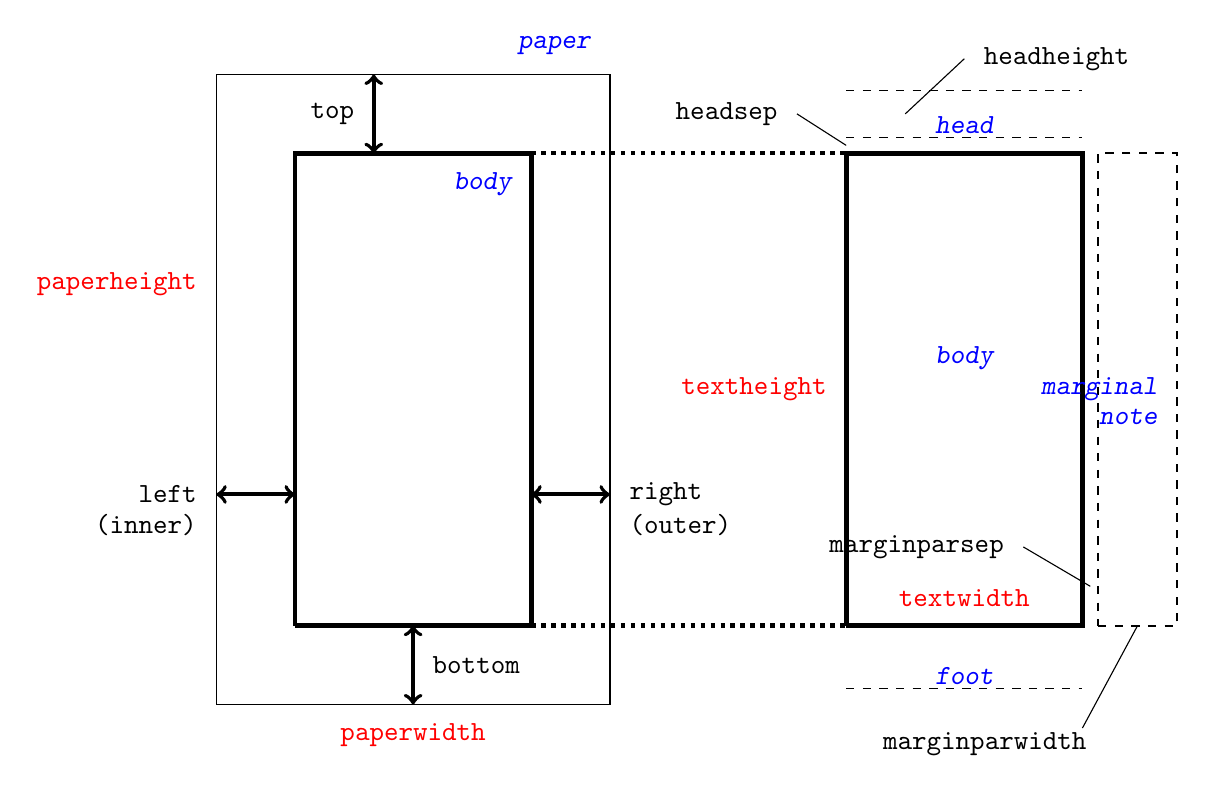
\begin{tikzpicture}{scale=0.9}
% outer-width & outer-height
\newcommand{\owd}{5};
\newcommand{\oht}{8};
% inner-width & inner-height
\newcommand{\iwd}{3};
\newcommand{\iht}{6};
% line length
\newcommand{\len}{5}

% Total Layout
\draw (0,0)--(\owd,0)--(\owd,\oht)--(0,\oht)--(0,0);
\draw[line width=0.06cm] (1,1)--(1+\iwd,1)--(1+\iwd,1+\iht)--(1,1+\iht)--(1,1);
\draw[ultra thick,dotted] (1+\iwd,1+\iht)--(\iwd+\len,1+\iht);
\draw[ultra thick,dotted] (1+\iwd,1)--(\iwd+\len,1);
% Arrow
\draw[<->,line width=0.05cm] (0,1/3*\oht)--(1,1/3*\oht);
\node[label=180:\texttt{left}] at (0,1/3*\oht){};
\node[label=225:\texttt{(inner)}] at (0,1/3*\oht){};
\draw[<->,line width=0.05cm] (1+\iwd,1/3*\oht)--(2+\iwd,1/3*\oht);
\node[label=0:\texttt{right}] at (2+\iwd,1/3*\oht){};
\node[label=315:\texttt{(outer)}] at (2+\iwd,1/3*\oht){};
\draw[<->,line width=0.05cm] (1+\iwd/2,1)--(1+\iwd/2,0);
\node[label=0:\texttt{bottom}] at (1+\iwd/2,0.5){};
\draw[<->,line width=0.05cm] (1+\iwd/3,1+\iht)--(1+\iwd/3,\oht);
\node[label=180:\texttt{top}] at (1+\iwd/3,1/2+\iht/2+\oht/2){};
% Outer Page Label
\node[label=135:\color{blue}{\ttfamily\slshape{paper}}] at (\owd,\oht){};
\node[label=225:\color{blue}{\ttfamily\slshape{body}}] at (1+\iwd,1+\iht){};

% Inner Page
\newcommand{\inn}{\iwd+\len};
\draw[line width=0.06cm] (\inn,1)--(\inn+\iwd,1)--(\inn+\iwd,1+\iht)--(\inn,1+\iht)--(\inn,1);
\node[label=180:\color{red}{\ttfamily{textheight}}] at (\inn,1+\iht/2){};
\node[label=90:\color{red}{\ttfamily{textwidth}}] at (\inn+\iwd/2,1){};
% Margin
\newcommand{\marsep}{0.2}
\newcommand{\marwd}{1}
\newcommand{\mar}{\inn+\iwd+\marsep}
\draw[thick,dashed] (\mar,1)--(\mar+\marwd,1)--(\mar+\marwd,1+\iht)--(\mar,1+\iht)--(\mar,1);
\draw (\mar-\marsep/2,1.5)--(\inn+3/4*\iwd,2);
\node[label=180:\texttt{marginparsep}] at (\inn+3/4*\iwd,2){};
\draw (\mar+\marwd/2,1)--(\inn+\iwd,-0.3);
\node[label=180:\texttt{marginparwidth}] at (\mar+\marsep/2,-0.5){};
% Foot
\draw[dashed] (\inn,0.2)--(\inn+\iwd,0.2);
\node[label=90:\color{blue}{\ttfamily\slshape{foot}}] at (\inn+\iwd/2,0){};
% Head
\draw[dashed] (\inn,1+\iht+0.8)--(\inn+\iwd,1+\iht+0.8);
\draw[dashed] (\inn,1+\iht+0.2)--(\inn+\iwd,1+\iht+0.2);
\node[label=90:\color{blue}{\ttfamily\slshape{head}}] at (\inn+\iwd/2,1+\iht){};
\draw (\inn,1+\iht+0.1)--(\inn-\len/8,1+\iht+0.5);
\node[label=180:\texttt{headsep}] at (\inn-\len/8,1+\iht+0.5){};
\draw (\inn+\iwd/4,1+\iht+0.5)--(\inn+\iwd/2,1+\iht+1.2);
\node[label=0:\texttt{headheight}] at (\inn+\iwd/2,1+\iht+1.2){};

% Total
\node[label=180:\color{red}{\ttfamily{paperheight}}] at (0,2/3*\oht){};
\node[label=270:\color{red}{\ttfamily{paperwidth}}] at (\owd/2,0){};
\node[label=\color{blue}{\ttfamily\slshape{body}}] at (\inn+\iwd/2,1+\iht/2){};
\node[label=180:\color{blue}{\ttfamily\slshape{marginal}}] at (\mar+\marwd,1+\iht/2){};
\node[label=225:\color{blue}{\ttfamily\slshape{note}}] at (\mar+\marwd,1+\iht/2){};
\end{tikzpicture}
\figcaption{页面构成示意图}
\label{fig:geo-paper}
\end{figure}

geometry宏包的具体的选项参数有:
\begin{feai}
\item \texttt{paper=<papername>:} 其中纸张尺寸有[a0--a6, b0--b6, c0--c6]paper, ansi[a--e]paper, letterpaper, executivepaper, legalpaper.
\item \texttt{papersize=\{<width>,<height>\}}: 自定义尺寸。也可以单独对paperwidth或者paperheigth赋值。
\item \texttt{landscape}: 切换到横向纸张。默认的是portrait.
\end{feai}

body部分分为两个概念:一个是总文本区(total body),另一个是主文本区(body). 总文本区可以由主文本区加上页眉(head)、页脚(foot)、侧页边(marginalpar)组成。默认的选项为includehead,表示总文本区包含页眉。要包括其他内容,可使用:\texttt{includefoot, includeheadfoot, includemp, includeall},以及以上各个参数将include改为ignore后的参数。

总文本区在默认状态下占纸张总尺寸的0.7,由scale=0.7控制,你也可以分别用\texttt{hscale}和\texttt{vscale}指定宽和高的占比。用具体的长度定义也是可以的,使用\texttt{(total)width}和\texttt{(total)height}定义总文本区尺寸,或者用\texttt{textwidth}和\texttt{textheight}定义主文本区的尺寸\footnote{当totalwidth和textwidth都定义时,优先采用后者的值。}。或者直接用\texttt{total=\{width,height\}, body=\{width,height\}}定义。甚至你可以用\texttt{lines=<num>}行数指定textheight。

页边的控制最为常用,分别用\texttt{left/inner, right/outer, top, bottom}来定义四向的页边。其中\texttt{inner, outer}参数只在文档的twoside参数启用时才有意义。你可以用\texttt{hmarginratio}来给定left(inner)与right(outer)页边宽的比例,默认是单页1:1、双页2:3。top和bottom之间的比由\texttt{vmarginratio}给定。你也可以用\texttt{vcentering, hcentering, centering}来指定页边比例为1:1. 在文档的左侧(内侧),可以指定装订线宽度\texttt{bindingoffset},使页边不会侵入。

页眉和页脚是位于top和bottom页边之内的文档元素。对于页眉和页脚的高度,分别使用\texttt{headheight/head, footskip/foot}参数指定。\texttt{marginpar}用来指定侧页边的宽度。它们到主文本区的参数分别是\texttt{headsep, footnotesep, marginparsep}. 你可以用\texttt{nohead, nofoot, nomarginpar}参数来清除总文本区中的页眉,页脚和侧页边。

对于在文档类documentclass命令中能使用的参数,geometry有不少也能做。比如\texttt{twoside, onecolumn, twocolumn}。甚至还能用文档类中不能用的\texttt{columnsep}(启用多栏分隔线)。

最后,这是几个小例子:
\begin{latex}{}
% 与Microsoft Word的默认样式相同:
\usepackage[hmargin=1.25in,vmargin=1in]{geometry}
% 书籍中靠书脊一侧的边距较小:
\usepackage[inner=1in,outer=1.25in]{geometry}
\end{latex}

\subsection{页眉和页脚}
主要借助fancyhdr宏包。\LaTeX 中的页眉页脚定义主要借助了两个命令,一个是\latexline{\\pagestyle},参数有:
\begin{para}
\item[empty] 无页眉页脚。
\item[plain] 无页眉,页脚只包含一个居中的页码。
\item[headings] 无页眉,页脚包含章/节名称与页码。
\item[myheadings] 无页眉,页脚包含页码和用户定义的信息。
\end{para}

另一个命令是\latexline{\\pagenumbering},与计数器一样,拥有\texttt{arabic, [Rr]oman, [Aa]lph}五种页码形式。

fancyhdr宏包给出了一个叫fancy的pagestyle,将页眉和页脚分别分为左中右三个部分,分别叫lhead, chead, rhead, 以及类似的[lcr]foot. 页眉页脚处的横线粗细也可以定义,默认页眉为0.4pt、页脚为0pt. 下面是一个例子:
\begin{latex}{}
\usepackage{fancyhdr}
\pagestyle{fancy}
  \lhead{}
  \chead{}
  \rhead{\bfseries wklchris}
  \lfoot{Leftfoot}
  \cfoot{\thepage}
  \rfoot{Rightfoot}
\renewcommand{\headrulewidth}{0.4pt}
\renewcommand{\footrulewidth}{0.4pt}
\end{latex}

加载这个宏包更多地是为了解决双页文档的排版问题。对于双页文档,fancyhdr宏包给出了一套新的指令:用E, O表示单数页和双数页,L, C, R表示左中右,H, F表示页眉和页脚。其中H, F需要配合\latexline{\\fancyhf}命令使用,比如\latexline{\\fancyhf[HC,FC]{This}}。如果不使用H, F参数,可以使用fancyhead, fancyfoot两个命令代替。一个新的例子:
\begin{latex}{}
\fancyhead{} % 清空页眉
  \fancyhead[RO,LE]{\bfseries wklchris}
\fancyfoot{} % 清空页脚
  \fancyfoot[LE,RO]{Leftfoot}
  \fancyfoot[C]{\thepage}
  \fancyfoot[RE,LO]{Rightfoot}
\end{latex}

fancyhdr在定义双页文档时,采用了如下的默认设置:
\begin{latex}{}
\fancyhead[LE,RO]{\slshape \rightmark}
\fancyhead[LO,RE]{\slshape \leftmark}
\fancyfoot[C]{\thepage}
\end{latex}

上例中的\latexline{\\rightmark}表示较低级别的信息,即当前页所在的section,形式如“1.2 sectionname ”,对于article则是subsection;而\latexline{\\leftmark}表示较高级别的信息,即对应的chapter,对于article则是section. 命令\latexline{\\leftmark}包含了页面上\latexline{\\markboth}\footnote{\latexline{\\markboth}是一个会被\latexline{\\chapter}等命令调用的命令,默认右参数是空。注意,带星号的大纲不调用这一命令,你需要这样书写:\latexline{\\chapter*{This\\markboth{This}{}}}。}下的最后一条命令的左参数,比如该页上出现了section 1--2,那么leftmark就是“Section 2”;命令\latexline{\\rightmark}则包含了页面上的第一个\latexline{\\markboth}命令的右参数或者第一个\latexline{\\markright}命令的唯一参数,比如可能是“Subsection 1.2”。

这听起来可能难以理解,但是markboth命令有两个参数,分别对应显示在文档的左页和右页(但是默认右参数留空,用markright命令去指定右页),故有左右之分;而markright命令只有一个参数。你可以试着再去理解一下双页文档下的fancyhdr的默认设置。利用这一点来重定义chaptermark, sectionmark, subsectionmark(仅其中两项)命令,举个例子:
\begin{latex}{}
% 这里的参数#1是指输入的section/chapter的标题
% 效果:“1.2. The section”
\renewcommand{\sectionmark}[1]{\markright{\thesection.\ #1}}
% 效果:“CHAPTER 2. The chapter”
\renewcommand{\chaptermark}[1]{\markboth{\MakeUppercase{%
  \chaptername}\ \thechapter.\ #1}{}}
\end{latex}

如果你对于默认的pagestyle不满意,可以用\latexline{\\fancypagestyle}命令进行更改。例如更改plain页面类型:
\begin{latex}{}
\fancypagestyle{plain}{
  \fancyhf{} % 清空页眉页脚
  \fancyhead[c]{\thesection}
  \fancyfoot{\thepage}}
\end{latex}

\section{抄录与代码环境}
抄录是指将键盘输入的字符(包括保留字符和空格)不经过\TeX 解释,直接输出到文档。默认的字体参数是等宽字族(ttfamily)。使用方法是\verb|\verb(*)|命令或者verbatim(*)环境,区别在于带星号的会将空格以“\textvisiblespace”(\latexline{\\textvisiblespace})的形式标记出来。

注意,\verb|\verb|命令是一个特殊的命令,可以用一组花括号括住抄录内容,也可以任意两个同样的符号(但不能是*)。比如:
\begin{latex}{}
\verb|fooo{}bar|
\verb+fooo{}bar+
\end{latex}

注意\latexline{\\verb(*)}以及verbatim(*)环境很脆弱,不能隐式地用于自定义环境,也一般不能用作命令的参数。verbatim宏包提供了更多的抄录支持,读者可自行查阅。

代码环境的输出,比如本文中带行号的代码块,参见\hyperref[sec:coding]{这一节}。

\section{分栏}
这部分内容使用\latexline{\\documentclass[twocolumn]{...}}这个可选参数就可以实现。在双栏模式下,\latexline{\\newpage}命令只会换栏,而\latexline{\\clearpage}命令才会换页。

如果在同一页内需要分栏与单栏并存(比如摘要跨栏,正文分栏),或者想要分三栏,请参考multicol宏包。

\section{文档拆分}
\label{sec:include}
文档拆分很简单,只需要把多个tex文件放在一起,然后再主文件中使用\latexline{\\input{filename.tex}}或者\latexline{\\include{filename}}命令就可以了,注意include不带扩展名。两个命令区别在于\latexline{\\include}命令将会很好地支持大纲编号。

拆分的优势在于可以根据chapter(或其他)分为多个文件,省去了长文档浏览时的一些不便。你也可以把整个导言区做成一个文件,然后在不同的\LaTeX 文档中反复使用,即充当模板的功能。你还可以把较长的tikz绘图代码写到一个tex中,在需要时\latexline{\\input}即可。

\section{西文排版及其他}
\subsection{连写}
\LaTeX 排版以及正规排版中,如果你输入ff, fl, fi, ffi等内容,它们默认会连写。在字母中间插入空白的箱子以强制不连写:\latexline{f\\mbox{}l}。

\subsection{断词}
行末的英文单词太长,\LaTeX 就会以其音节断词。如果你想指定某些单词的断词位置,使用如下命令断词。例子:
\begin{latex}{}
\hyphenation{Hy-phen-a-tion FORTRAN}
\end{latex}

这个例子允许Hyphenation, hyphenation在短横处断词,同时\textbf{禁止}FORTRAN, Fortran, fortran断词。如果你在行文中加入\verb|\-|命令,则可以实现允许在对应位置断词的效果。比如:

\begin{codeshow}
I will show you this example:
su\-per\-cal\-i\-frag\-i\-lis\-%
tic\-ex\-pi\-al\-i\-do\-cious
\end{codeshow}

如果你不想断词,比如电话号码,巧妙利用\latexline{\\mbox}命令吧:
\begin{latex}{}
My telephone number is: \mbox{012 3456 7890}
\end{latex}

\subsection{特殊符号}
符号的总表可以参照symbols-a4文档,运行texdoc symbols-a4即可调出。包括希腊字母在内的一些数学符号将会在下一章介绍。这里给出基于wasysym宏包的一些常用符号:
\begin{center}
  \centering
  \tabcaption{wasysym宏包符号}
  \begin{tabular}{*{3}{c >{\ttfamily\char92}p{5.5em}}}
     \permil     & permil   & \male     & male  & \female       & female \\
     \checked    & checked  & \XBox     & XBox  & \CheckedBox   & CheckedBox \\
     \hexstar    & hexstar  & \phone    & phone & \twonotes     & twonotes
  \end{tabular}
\end{center}

\subsection{其他}
如果你想在某个不带参数的命令后输入空格,请接上一个空的花括号确保空格能够正常输出。例如:\latexline{这是\\TeX{} Live. }

\chapter{数学排版}
\section{行间与行内公式}
\co{行内公式}指将公式嵌入到文段的排版方式,主要要求公式垂直距离不能过高,否则影响排版效果。行内公式的书写方式:
\begin{latex}{}
$...$ 或者 \(...\) 或者 \begin{math}...\end{math}
\end{latex}

一般推荐第一种方式。例如:\verb|$\sum_{i=1}^{n}a_i$|,即:$\sum_{i=1}^{n}a_i$.

另外一种公式排版方式是\co{行间公式},也称行外公式,使用:
\begin{latex}{}
\[...\] 或者 \begin{displaymath}...\end{displaymath}
或者 amsmath 提供的\begin{equation*}...\end{equation*}
\end{latex}

一般也推荐第一种命令\footnote{还有一种\texttt{\$\$...\$\$}的写法,问题很多,绝不建议使用。},例如:\verb|\[\sum_{i=1}^n{a_i}\]|,得到:

\[\sum_{i=1}^{n}a_i\]

从上面的两个例子可以看出,即使输出相同的内容,行内和行间的排版也是有区别的,比如累计符号上标是写在正上方还是写在右上角。

如果行间公式需要编号,使用equation环境\footnote{需要注意有一个\RED{已经淘汰}的多行公式编号环境叫\texttt{eqnarray},请不要再使用。},还可以插入标签:

\begin{codeshow}
\begin{equation}
\label{eq:NoExample}
  |\epsilon|>M
\end{equation}
\end{codeshow}

\section{数学字体、字号与空格}
\label{sec:mathfont}
\subsection{空格}
在数学环境中,行文空格是被忽略的。比如\verb|$x,y$|和\verb|$x, y$|并没有区别。数学环境有独有的空格命令,最后一个是$-3/18$的空格:

\begin{codeshow}
  $没有空格,3/18空\,格$ \\
  $4/18空\:格,5/18空\;格$ \\
  $9/18空\ 格,一个空\quad 格$ \\
  $两个空\qquad 格,负3/18空\!格$
\end{codeshow}

事实上,以上命令也可以在数学模式外使用,其中使用最广泛的是\verb|\,|,比如上文提到过的千位分隔符。在数学环境中它也应用广泛:

\begin{codeshow}
\[ \int_0^1 x \ud{}x
= \frac{1}{2} \]
\end{codeshow}

其中\verb|\ud|命令是自定义的,这也是微分算子的正常定义\label{cmd:ud}:
\begin{latex}{}
\newcommand{\ud}{\mathop{}\negthinspace\mathrm{d}}
\end{latex}

\subsection{数学字号}
\LaTeX{}提供四种字号尺寸命令:
\begin{para}
\item[\char92 displaystyle:] 行间公式尺寸。如$\displaystyle \sum_{i=1}^n a$
\item[\char92 textstyle:] 行内公式尺寸。如$\textstyle \sum_{i=1}^n a$
\item[\char92 scriptstyle:] 上下标尺寸。如$\scriptstyle \sum_{i=1}^n a$
\item[\char92 scriptscriptstyle:] 次上下标尺寸。如$\scriptscriptstyle \sum_{i=1}^n a$
\end{para}

\subsection{数学字体}
将字体转为正体使用\latexline{\\mathrm}命令。如需保留文中空格,使用\latexline{\\textrm}命令——这个与正文一致。但是,textrm命令内的字号可能不会自适应,mathrm则稳定得多。

例如自然对数的底数$\ue$,在本文中就是这样定义的:
\begin{latex}{}
\newcommand{\ue}{\mathrm{e}}
\end{latex}

以下简单介绍几种数学字体。数学字体的总表参见\tref{tab:mathfont}。

\subsubsection{数学粗体}
数学粗体使用amsmath宏包支持的\latexline{\\boldsymbol}命令。命令\latexline{\\boldmath}的问题在于它只能加粗一个数学环境,其中很可能包括了标点符号,而这是不严谨的。命令\latexline{\\mathbf}就差的更远,它只能把字体转为\textbf{正}粗体,而数学字体都是斜体的。

\begin{codeshow}
$\mu,M$\\
$\boldsymbol{\mu},
\boldsymbol{M}$ \\
\end{codeshow}

\subsubsection{空心粗体}
空心粗体使用amsfonts或amssymb宏包的\latexline{\\mathbb}命令。这里用\latexline{\\textrm}而不是\latexline{\\mathrm},是为了保留空格。

\begin{codeshow}
$x^2 \geq 0 \qquad
\textrm{for all }x\in\mathbb{R}$
\end{codeshow}

\section{基本命令}
基本函数默认用正体书写,包括:
\begin{verbatim}
\sin \cos \tan \cot \arcsin \arccos \arctan \cot \sec \csc
\sinh \cosh \tanh \coth \log \lg \ln \ker \exp \dim \arg \deg 
\lim \limsup \liminf \sup \inf \min \max \det \Pr \gcd
\end{verbatim}

以上函数,最后一行的10个是可以带上下限参数的,即在行间公式模式下,上标和下标将在函数正上方和正下方书写内容。

amsmath宏包允许\latexline{\\DeclareMathOperator}命令自定义基本函数;如果命令带星号,则可以带上下限参数。

此外有一个叫\latexline{\\mathop}的命令,可以把任何的数学字符串转换为数学对象,使其适用上标、下标等数学对象才能使用的命令。

\subsection{上下标与虚位}
用低划线和尖角符表示上标和下标,请仔细体会下述例子:

\begin{codeshow}
$a^3_{ij}$ \\
${a_{ij}}^3\text{或}a_{ij}{}^3$\\
$\mathrm{e}^{x^2}\geq 1$
\end{codeshow}

上面的指数3的位置读者可以多多体会一下。此外,\verb|\phantom|被称为虚位命令,从下例你也能够体会到他的作用:

\begin{codeshow}
${}^{12}_{6}\mathrm{C}$ \\
${}^{12}_{\phantom{1}6}
\mathrm{C}$ \\
$a^3_{ij}$ \\
$a^{\phantom{ij}3}_{ij}$
\end{codeshow}

\subsection{微分与积分}
导数直接使用单引号\verb|'|,积分使用\verb|\int|符号:

\begin{codeshow}
$y'=x \qquad \dot{y}(t)=t$ \\
$\ddot{y}(t)=t+1$
$\dddot{y}+\ddddot{y}=0$ \\
$\iint_{D}f(x)=0$
$\int_{0}^{1}f(x)=1$
\end{codeshow}

有时候需要更高级的微分或积分号,其中\latexline{\\ud}命令在\hyperref[cmd:ud]{上文这里}定义过:
\begin{latex}{}
\[\left.\frac{\ud y}{\ud x}\right|_{x=0}
\quad\frac{\partial f}{\partial x}
\quad\oint\;\varoiint_S \]
\end{latex}

效果:
\[\left.\frac{y}{x}\right|_{x=0}
\quad\frac{\partial f}{\partial x}\quad
\oint\;\varoiint_S \]

其中的\verb|\dot|系的导数形式\LaTeX 只原生支持到二阶导数。后面的三阶、四阶需要amsmath宏包。\verb|\int|系的积分命令也是一样。而环形双重积分命令\verb|\varoiint|需要esint宏包\footnote{该宏包可能与amsmath冲突,即便使用也请其放在amsmath之后加载。}。

\verb|\left.|或\verb|\right.|命令\footnote{参考\hyperref[subsec:delimiter]{定界符}部分的内容。}只用于匹配,本身不输出任何内容。

\subsection{分式、根式与堆叠}
分式使用\verb|\frac|命令。或者amsmath宏包支持的\latexline{\\dfrac}命令来强制获得行间公式大小的分数,\latexline{\\tfrac}则强制获得行内公式大小的分数:

\begin{codeshow}
$\sqrt{\frac{x}{y}}$ \\
$x^{1/2} \qquad x^{\frac{2}{3}}$\\
$\tfrac{1}{2}$ \quad $\dfrac{1}{2}$
\end{codeshow}

根式:

\begin{codeshow}
$\sqrt{2} \quad \surd$ \\
$\sqrt[3]{\sqrt{2}+1}$
\end{codeshow}

划线命令使用\verb|\underline|和\verb|\overline|,水平括号使用brace:

\begin{codeshow}
$\overline{m+n}$ \\
$\underbrace{a_1+\ldots+a_n}_{n}$
$\overbrace{a_1+\ldots+a_n}^{n}$
\end{codeshow}

事实上\verb|\overline|命令也存在问题,请比较:

\begin{codeshow}
$\overline{A}\overline{B}$ \\
$\closure{A}\closure{B}$
$\closure{AB}$
\end{codeshow}

其中closure是在导言区定义的
\begin{latex}{}
\newcommand{\closure}[2][3]{{}\mkern#1mu
  \overline{\mkern-#1mu#2}}
\end{latex}

向量符号:

\begin{codeshow}
  $\vec a\quad\overrightarrow{PQ}$
  $\overleftarrow{EF}$
\end{codeshow}

尖帽符号或者波浪符号:

\begin{codeshow}
  $\hat{A} \quad \widehat{AB}$ \\
  $\tilde{C} \quad \widetilde{CD}$
\end{codeshow}

强制堆叠命\latexline{\\stackrel},位于上方的符号与上标同等大小。如果有amsmath宏包,可以使用\latexline{\\overset}或者\latexline{\\underset} 命令,前者与\latexline{\\stackrel}命令完全等同:

\begin{codeshow}
  $\int f(x) \stackrel{?}{=} 1$\\
  $A\overset{abc}{=}B$ \quad
  $C\underset{def}{=}D$
\end{codeshow}

还有一个很强大的堆叠放置命令\verb|\sideset|:

\begin{codeshow}
\[\sideset{_a^b}{_c^d}\sum\]
\[\sideset{}{'}\sum_{n=1}\text{或}
\,{\sum\limits_{n=1}}'\]
\end{codeshow}

去心邻域大概也属于堆叠符的一种?这样输出:

\begin{codeshow}
$\mathring{U}$
\end{codeshow}

在下一次节:累加与累积中,还介绍了更多的堆叠命令。

\subsection{累加与累积}
使用\verb|\sum|和\verb|\prod|命令,效果如下:

\begin{codeshow}
\[\sum_{i=1}^{n}a_i=1 \qquad
\prod_{j=1}^{n}b_j=1\]
\end{codeshow}

有时需要复杂的堆叠方式,效果如下:

\begin{codeshow}
\[\sum_{\substack{0<i<n \\
  0<j<m}} p_{ij}=
  \prod_{\begin{subarray}{l}
  i\in I \\  1<j<m
  \end{subarray}}q_{ij}\]
\end{codeshow}

有时候需要强制实现堆叠的效果,可以使用\latexline{\\limits}命令。如果堆积目标不是数学对象,还需要使用\latexline{\\mathop}命令:

\begin{codeshow}
\[\max\limits_{i>1}^{x}\quad
\mathop{xyz}\limits_{x>0}\quad
\lim\nolimits_{x\to \infty}\]
\end{codeshow}

\subsection{矩阵与省略号}
矩阵的排版可以通过array环境和自适应定界符完成:

\begin{codeshow}
\[\mathbf{A}=
\left(\begin{array}{ccc}
x_{11} & x_{12} & \ldots \\
x_{21} & x_{22} & \ldots \\
\vdots & \vdots & \ddots
\end{array}\right)\]
\end{codeshow}

还有就是\verb|\cdots|命令。hmath宏包还提供了一种省略号\verb|\adots|:$\adots$,或许用得上呢?

\LaTeX 原生支持自动添加定界符的形式,不过要放在数学环境内:

\begin{codeshow}
\centering $\begin{matrix}
0 & 1 \\ 1 & 0 \end{matrix}\qquad
\begin{pmatrix} 0 & 2 \\
2 & 0 \end{pmatrix}$
\end{codeshow}

方括号和花括号使用\verb|\bmatrix|命令:

\begin{codeshow}
\centering $\begin{bmatrix}
0 & 3 \\ 3 & 0 \end{bmatrix}\qquad
\begin{Bmatrix} 0 & 4 \\
4 & 0 \end{Bmatrix}$
\end{codeshow}

行列式使用\verb|\vmatrix|命令:

\begin{codeshow}
\centering $\begin{vmatrix}
0 & 5 \\ 5 & 0 \end{vmatrix}\qquad
\begin{Vmatrix} 0 & 6 \\
6 & 0 \end{Vmatrix}$
\end{codeshow}

在矩阵中排版dfrac分式时,使用在换行符后添加竖直空距的方法解决行距问题:

\begin{codeshow}
\[\mathbf{H}=
\begin{bmatrix}
\dfrac{\partial^2 f}{\partial x^2} &
\dfrac{\partial^2 f}
{\partial x \partial y} \\[8pt]
\dfrac{\partial^2 f}
{\partial x \partial y} &
\dfrac{\partial^2 f}{\partial y^2}
\end{bmatrix}\]
\end{codeshow}


\subsection{分段函数与联立方程}
array也可以用来写分段函数:

\begin{codeshow}
\[y=\left\{\begin{array}{ll}
x+1, & x>0 \\
0,   & x=0 \\
x-1, & x<0
\end{array}\right.\]
\end{codeshow}

分段函数还能用cases环境,它自动生成一个花括号,也更紧凑:

\begin{codeshow}
\[y=\begin{cases}
\int x, & x>0 \\
0,   & x=0 \\
x-1, & x<0
\end{cases},\,
x\in\mathbb{R}\]
\end{codeshow}

如果想要生成display样式的内容(比如上面的积分号只是text样式的),使用mathtools宏包的dcases环境代替cases环境。如果cases环境的第二列条件不是数学语言而是一般文字,可以考虑使用dcases*环境,列中用\&{}隔开。

\begin{codeshow}
\[y=\begin{dcases}
  \int x, & x>0 \\
  x^2, & x\leqslant 0
  \end{dcases}\]
\[z=\begin{dcases*}
  y, & when $y$ is prime\\
  y^2, & otherwise
  \end{dcases*}\]
\end{codeshow}

\subsection{多行公式及其编号}
\label{subsec:multieqnum}
多行公式可以使用amsmath下的align环境——因为原生的eqnarray环境真的很差!而且align环境不需要像array环境那样给出列的数目和参数,能够根据
\texttt{\&}符号的数量来自调整。\qd{这个环境会自动对齐等号或者不等号,所以必要时请用\&指定对齐位置}。下面是一个例子:

\begin{codeshow}
\begin{align}
  a^2  &= a\cdot a \\
       &= a*a      \\
       &= a^2
\end{align}
\end{codeshow}

\LaTeX 中长公式不能自动换行\footnote{不过breqn宏包的dmath环境可以实现自动换行,读者可以自行尝试。},请自行指定断行位置和缩进距离,就像上面一样。也许你不需要三个编号,你可以:

\begin{codeshow}
\begin{align}
  a^2&= a\cdot a& b&=c\nonumber\\
  g  &= a*a & d&>e>f  \nonumber\\
  step&= a^2 & &Z^3
\end{align}
\end{codeshow}

如果你想让编号显示在这三行的中间而不是最下面一行,可以尝试把公式写在aligned或者gathered环境中,然后再嵌套到equation环境内。如果你根本不想给多行公式编号,尝试align*环境。

另外,amsmath宏包的multline环境将自动把编号放在末行。首行左对齐,末行右对齐,中间的行居中。

如果想在环境中插入小段行间文字,使用intertext命令,或者mathtools宏包的shortintertext命令。区别是后者的垂直间距更小一些。

\begin{codeshow}
\begin{align*}
\shortintertext{If}
 y &= 0 \\
 x &< 0\\
\shortintertext{then}
 z &= x+y
\end{align*}
\end{codeshow}

当然,align环境是用来分列对齐的。如果你仅仅想要所有行居中,使用amsmath宏包的gather环境即可。这是一个非常实用的环境,你也可以用gather*环境排版居中的、非编号的多行公式。

\begin{codeshow}
\begin{gather}
  X=1+2+\cdots+n \\
  Y=1
\end{gather}
\end{codeshow}

\subsection{二项式与定理}
二项式可能需要借助amsmath宏包的\verb|\binom|命令:

\begin{codeshow}
  $\mathrm{C}_n^k=\binom{n}{k}$
\end{codeshow}

\RED{在使用这部分内容时,请加载amsthm宏包}。

首先是定理环境格式的自定义。如同定义命令一样,在导言区加上:

\noindent\begin{tabular}{|l|}
\hline
\char92{}newtheorem\{\textit{name}\}[\textit{counter}]\{\textit{text}\}[\textit{section}] \\
\hline
\end{tabular}

其中\textit{name}表示定理的引用名称,即下文将其作为一个环境名来识别;\textit{text}表示定理的显示名称,即下文中定理将以其作为打印内容。而\textit{counter}参数表示你是否与先前声明的某定理共同编号。\textit{section}参数表示定理的计数层级,如果是section,表示每节分别计数;chapter表示每章分别计数。

来看一个例子。首先在导言区定义如下三个样式:
\begin{verbatim}
\theoremstyle{definition}\newtheorem{laws}{Law}[section]
\theoremstyle{plain}\newtheorem{ju}[laws]{Jury}
\theoremstyle{remark}\newtheorem*{marg}{Margaret}
\end{verbatim}

以上三个theoremstyle即是它预定义的所有样式类型。definition标题粗体,内容罗马体;plain标题粗体,内容斜体;remark标题斜体,内容罗马体。带星号表示不进行计数。在环境的使用中可以添加可选参数,用于以括号的形式注释定理。然后这是示例:

\begin{codeshow}
\begin{laws}
Never believe easily.
\end{laws}
\begin{ju}[The 2nd]
Never suspect too much.
\end{ju}
\begin{marg}Nothing else.\end{marg}
\end{codeshow}

amsthm宏包也提供了proof环境,并且用\latexline{\\qedhere}来指定证毕符号的位置。如果不加指定,将会自动另起一行。

\begin{codeshow}
\begin{proof}
For an right triangle, we have:
  \[a^2+b^2=c^2 \qedhere\]
\end{proof}
\end{codeshow}

\section{数学符号与字体}
\subsection{数学字体}
原生的数学字体命令:
\begin{center}
\tabcaption{原生数学字体表}
\label{tab:mathfont}
\begin{tabular}{>{\ttfamily\char92}l>{$}l<{$}}
\hline
mathrm\{ABCDabcde 1234\} & \mathrm{ABCDabcde 1234} \\
\hline
mathit\{ABCDabcde 1234\} & \mathit{ABCDabcde 123} \\
\hline
mathnormal\{ABCDabcde 1234\} & \mathnormal{ABCDabcde 1234} \\
\hline
mathcal\{ABCDabcde 1234\} & \mathcal{ABCDabcde 1234} \\
\hline
\end{tabular}
\end{center}

需要其他宏包支持的数学字体:
\begin{center}
\tabcaption{宏包数学字体表}
\label{tab:mathfont-pk}
\begin{tabular}{>{\ttfamily}ll}
\hline
\char92mathscr\{ABCDabcde 1234\} & mathrsfs\\
$\mathscr{ABCDabcde 1234}$ & \\
\hline
\char92mathfrak\{ABCDabcde 1234\} & amsfonts或者amssymb\\
$\mathfrak{ABCDabcde 1234}$ & \\
\hline
\char92mathbb\{ABCDabcde 1234\} & amsfonts或者amssymb\\
$\mathbb{ABCDabcde 1234}$ & \\
\hline
\end{tabular}
\end{center}

\subsection{定界符}
\label{subsec:delimiter}
\tref{tab:delimiter}给出了一些数学环境中使用的定界符。

\begin{table}[!htb]
\centering
\caption{定界符}
\label{tab:delimiter}
\begin{tabular}{@{}*{3}{>{$}p{2em}<{$} @{} >{\ttfamily}p{7em}}}
( & ( & [ & [ or \char92 lbrack & \uparrow & \char92 uparrow \\
) & ) & ] & ] or \char92 rbrack & \downarrow & \char92 downarrow \\
\{ & \{ or \char92 lbrace & \} & \} or \char92 rbrace & \updownarrow & \char92 updownarrow \\
\langle & \char92 langle & \rangle & \char92 rangle & \backslash & \char92 backslash \\
\lfloor & \char92 lfloor & \rfloor & \char92 rfloor & \Updownarrow & \char92 Updownarrow \\
\lceil & \char92 lceil & \rceil & \char92 rceil & \Uparrow & \char92 Uparrow \\
\Vert & \char92 | or \char92 Vert & | & | or \char92 vert & \Downarrow & \char92 Downarrow \\
\hline
\multicolumn{6}{c}{-- 以下需要amssymb宏包 --} \\
\multicolumn{3}{c}{$\ulcorner$ \quad \texttt{\char92 ulcorner}} & \multicolumn{3}{c}{$\urcorner$ \quad \texttt{\char92 urcorner}} \\
\multicolumn{3}{c}{$\llcorner$ \quad \texttt{\char92 llcorner}} & \multicolumn{3}{c}{$\lrcorner$ \quad \texttt{\char92 lrcorner}}
\end{tabular}
\end{table}

使用\verb|\left|或者\verb|\right|能够使定界符自适应式子的高度:

\begin{codeshow}
\[\left\{x+\frac{\left[\left|\frac
{y}{x}\right|^3-Z^{5\left(\frac{x}
{y}+z\right)}\right]}{y}\right\}\]
\end{codeshow}

有时\verb|\left.|和\verb|\right.|能灵活地用于跨行控制,因为它们并非实际配对:

\begin{codeshow}
\begin{align*}
  x &=\left(\frac{1}{2}x\right.\\
  &\left.\vphantom{\frac{1}{2}}
  +y^2+z_1\right)
\end{align*}
\end{codeshow}

其中\verb|\vphantom|命令用于输出一个高度虚位,使得第二行的自适应定界符与第一行同等大小。

有时你可能希望手动指定定界符的尺寸,这时使用:

\begin{codeshow}
  $(\big(\Big(\bigg(\Bigg($ \\
  \[\bigl[\frac{x+y}{x^2}\bigr]\]
\end{codeshow}

\subsection{希腊字母}
希腊字母表如\tref{tab:greekletter}所示。表中包含了小写希腊字母、大写希腊字母,其中部分希腊字母的输入方式与英文字母一致。
\begin{table}[!htb]
\centering
\caption{希腊字母表}
\label{tab:greekletter}
\begin{tabular}{*{4}{>{$}p{2em}<{$} @{} >{\ttfamily\char92}p{6em} @{}}}
\alpha & alpha & \theta & theta & o & \multicolumn{1}{p{6em}}{o} & \upsilon & upsilon \\
\beta & beta & \vartheta & vartheta & \pi & pi & \phi & phi \\
\gamma & gamma & \iota & iota & \varpi & varpi & \varphi & varphi \\
\delta & delta & \kappa & kappa & \rho & rho & \chi & chi \\
\epsilon & epsilon & \lambda & lambda & \varrho & varrho & \psi & psi \\
\varepsilon & varepsilon & \mu & mu & \sigma & sigma & \omega & omega \\
\zeta & zeta & \nu & nu & \varsigma & varsigma & \eta & eta \\
\xi & xi & \tau & tau & \multicolumn{4}{c}{} \\
A & \multicolumn{1}{p{6em}}{A} & B & \multicolumn{1}{p{6em}}{B} & \Gamma & Gamma & \varGamma & varGamma \\
\Delta & Delta & \varDelta & varDelta & E & \multicolumn{1}{p{6em}}{E} & Z & \multicolumn{1}{p{6em}}{Z} \\
H & \multicolumn{1}{p{6em}}{H} & \Theta & Theta & \varTheta & varTheta & I & \multicolumn{1}{p{6em}}{I} \\
\Lambda & Lambda & \varLambda & varLambda & M & \multicolumn{1}{p{6em}}{M} & N & \multicolumn{1}{p{6em}}{N} \\
\Xi & Xi & \varXi & varXi & O & \multicolumn{1}{p{6em}}{O} & \Pi & Pi \\
\varPi & varPi & P & \multicolumn{1}{p{6em}}{P} & \Sigma & Sigma & \varSigma & varSigma \\
T & \multicolumn{1}{p{6em}}{T} & \Upsilon & Upsilon & \varUpsilon & varUpsilon & \Phi & Phi \\
\varPhi & varPhi & X & \multicolumn{1}{p{6em}}{X} & \Psi & Psi & \varPsi & varPsi \\
\Omega & Omega & \varOmega & varOmega & \multicolumn{4}{c}{}
\end{tabular}
\end{table}

\subsection{二元运算符}
二元运算符包括常见的加减乘除,还有集合的交、并、补等运算。\tref{tab:operator}只列出常用的二元运算符,更多的请参考symbols-a4文档。
\begin{table}[!htb]
\centering
\caption{二元运算符}
\label{tab:operator}
\begin{tabular}{@{}*{2}{>{$}p{2em}<{$} @{} >{\ttfamily\char92}p{5em} @{}}*{2}{>{$}p{2em}<{$} @{} >{\ttfamily\char92}p{6em} @{}}}
+ & \multicolumn{1}{p{6em}}{+} & - & \multicolumn{1}{p{6em}}{-} & \times & times & \div & div \\
\pm & pm & \mp & mp & \circ & circ & \triangleright & triangleright \\
\cdot & cdot & \star & star & \ast & ast & \triangleleft & triangleleft \\
\cup & cup & \cap & cap & \setminus & setminus & \bullet & bullet \\
\oplus & oplus &\ominus & ominus & \otimes & otimes & \oslash & oslash \\
\odot & odot & \bigcirc & bigcirc & \vee & vee,lor & \wedge & wedge,land \\
\bigcup & bigcup & \bigcap & bigcap & \bigvee & bigvee & \bigwedge & bigwedge
\end{tabular}
\end{table}

\subsection{二元关系符}
二元关系符常常被用于判断两个数的大小关系,或者集合中的从属关系。\tref{tab:relation-operator}和\tref{tab:amsrelation-operator}只列出常用的二元关系符,更多的请参考symbols-a4文档。
\begin{table}[!htb]
\centering
\caption{二元关系符}
\label{tab:relation-operator}
\begin{tabular}{@{}*{4}{>{$}p{2em}<{$} @{} >{\ttfamily\char92}p{6em} @{}}}
< & \multicolumn{1}{p{6em}}{<} & > & \multicolumn{1}{p{6em}}{>} & \le & le(q) & \ge & ge(q) \\
\ll & ll & \gg & gg & \equiv & equiv & \neq & neq \\
\prec & prec & \succ & succ & \preceq & preceq & \succeq & succeq \\
\sim & sim & \simeq & simeq & \cong & cong & \approx & approx \\
\subset & subset & \supset & supset & \subseteq & subseteq & \supseteq & supseteq \\
\in & in & \ni & ni & \notin & notin & \propto & propto \\
\parallel & parallel & \perp & perp & \smile & smile & \frown & frown \\
\asymp & asymp & \bowtie & bowtie & \vdash & vdash & \dashv & dashv
\end{tabular}
\end{table}

\tref{tab:amsrelation-operator}中的二元关系符需要amssymb宏包。
\begin{table}[!htb]
\centering
\caption{amssymb二元关系符}
\label{tab:amsrelation-operator}
\begin{tabular}{@{}*{4}{>{$}p{2em}<{$} @{} >{\ttfamily\char92}p{6em} @{}}}
\leqslant & leqslant & \geqslant & geqslant & \because & because & \therefore & therefore \\
\nless & nless & \ngtr & ngtr & \lessdot & lessdot & \gtrdot & gtrdot \\
\lessgtr & lessgtr & \gtrless & gtrless & \lesseqqgtr & lesseqqgtr & \gtreqqless & gtreqqless \\
\subseteqq & subseteqq & \supseteqq & supseteqq & \subsetneqq & subsetneqq & \supsetneqq & supsetneqq
\end{tabular}
\end{table}

\subsection{箭头}
在\tref{tab:delimiter}中给出了几个箭头符号,但是不够全,这里给出总表如\tref{tab:arrow}。
\begin{table}[!htb]
\centering
\caption{箭头}
\label{tab:arrow}
\begin{tabular}{@{}*{2}{>{$}p{3em}<{$} @{} >{\ttfamily\char92}p{10em} @{}}}
\leftarrow & leftarrow & \longleftarrow & longleftarrow \\
\rightarrow & rightarrow & \longrightarrow & longrightarrow \\
\leftrightarrow & leftrightarrow & \longleftrightarrow & longleftrightarrow \\
\Leftarrow & Leftarrow & \Longleftarrow & Longleftarrow \\
\Rightarrow & Rightarrow & \Longrightarrow & Longrightarrow \\
\Leftrightarrow & Leftrightarrow & \Longleftrightarrow & Longleftrightarrow \\
\mapsto & mapsto & \longmapsto & longmapsto \\
\nearrow & nearrow & \searrow & searrow \\
\swarrow & swarrow & \nwarrow & nwarrow \\
\leftharpoonup & leftharpoonup & \rightharpoonup & rightharpoonup \\
\leftharpoondown & leftharpoondown & \rightharpoondown & rightharpoondown \\
\rightleftharpoons & rightleftharpoons & \iff & iff (bigger space)
\end{tabular}
\end{table}

依旧给出一个基于amssymb宏包的附\tref{tab:amsarrow}。
\begin{table}[!htb]
\centering
\caption{amssymb箭头}
\label{tab:amsarrow}
\begin{tabular}{@{}*{2}{>{$}p{3em}<{$} @{} >{\ttfamily\char92}p{10em} @{}}}
\dashleftarrow & dashleftarrow & \dashrightarrow & dashrightarrow \\
\circlearrowleft & circlearrowleft & \circlearrowright & circlearrowright \\
\leftrightarrows & leftrightarrows & \rightleftarrows & leftrightarrows \\
\nleftarrow & nleftarrow & \nLeftarrow & nLeftarrow \\
\nrightarrow & nrightarrow & \nRightarrow & nRightarrow \\
\nleftrightarrow & nleftrightarrow & \nLeftrightarrow & nLeftrightarrow
\end{tabular}
\end{table}

\subsection{其他符号}
最后是一些其他的难以归类的符号,也不全是数学领域会用到的,只不过它们可以在数学环境下输出出来,以及被amssymb宏包所支持。如\tref{tab:othersym}和\tref{tab:amsothersym}。
\begin{table}[!htb]
\centering
\caption{其他符号}
\label{tab:othersym}
\begin{tabular}{@{}*{4}{>{$}p{1em}<{$} @{} >{\ttfamily\char92}p{5.5em} @{}}}
\dots & dots & \cdots &cdots &
\vdots & vdots & \ddots & ddots \\
\forall & forall & \exists & exists &
\Re & Re & \aleph & aleph \\
\angle & angle & \infty & infty &
\triangle & triangle & \nabla & nabla \\
\hbar & hbar & \imath & imath &
\jmath & jmath & \ell & ell \\
\spadesuit & spadesuit & \heartsuit & heartsuit &
\clubsuit & clubsuit & \diamondsuit & diamondsuit \\
\flat & flat & \natural & natural &
\sharp & sharp & & \\
\hline
\multicolumn{8}{l}{非数学符号:} \\
\multicolumn{1}{p{2em}}{\pounds} & pounds & \multicolumn{1}{p{2em}}{\S} & S &
\multicolumn{1}{p{2em}}{\copyright} & copyright & \multicolumn{1}{p{2em}}{\P} & P \\
\multicolumn{1}{p{2em}}{\dag} & dag & \multicolumn{1}{p{2em}}{\ddag} & ddag &
\multicolumn{1}{p{2em}}{\textregistered} & \multicolumn{3}{l}{textregistered}
\end{tabular}
\end{table}

\begin{table}[!htb]
\centering
\caption{amssymb其他符号}
\label{tab:amsothersym}
\begin{tabular}{@{} >{$}p{2em}<{$} @{} >{\ttfamily\char92}p{6em} @{}*{2}{>{$}p{2em}<{$} @{} >{\ttfamily\char92}p{8em} @{}}}
\square & square & \blacksquare & blacksquare & \hslash & hslash \\
\bigstar & bigstar & \blacktriangle & blacktriangle & \blacktriangledown & blacktriangledown \\
\lozenge & lozenge & \blacklozenge & blacklozenge & \measuredangle & measuredangle \\
\mho & mho & \varnothing & varnothing & \eth & eth
\end{tabular}
\end{table}

\clearpage
\chapter{\LaTeX{}进阶}
本章的内容多数与宏包的使用相关。记得使用texdoc命令查看宏包的使用手册,这是学习宏包最好的手段,没有之一。

\section{自定义命令与环境}
\label{sec:newcommand}
自定义命令是\LaTeX 相比于字处理软件MS Word之流最强大的功能之一。它可以大幅度优化你的文档体积,用法是:
\begin{latex}{}
\newcommand{cmd}[args][default]{def}
\end{latex}

现在来解释一下各个参数:
\begin{para}
\item[cmd:] 新定义的命令,不能与现有命令重名。
\item[args:] 参数个数。
\item[default:] 首个参数,即\texttt{\#{}1}的默认值。
\item[def:] 具体的定义内容。参数1以\texttt{\#{}1}代替,参数2以\texttt{\#{}2}代替,以此类推。
\end{para}

如果重定义一个现有命令,使用\latexline{\\renewcommand}命令,用法与\latexline{\\newcommand}一致。简单的例子:
\begin{latex}{}
% 加粗:\concept{text}
\newcommand{\concept}[1]{\textbf{#1}}
% 加粗#2并把#1#2加入索引,默认#1为空。
% 比如\cop{Sys}或者\cop[Sec.]{Sys}
\newcommand{\cop}[2][]{\textbf{#2}}\index{#1 #2}}
\end{latex}

\section{箱子:排版的基础}
\label{sec:box}
\LaTeX 排版的基础单位就是“箱子(box)”,例如整个页面是一个矩形的箱子,侧边栏、主正文区、页眉页脚也都是箱子。在正常排版中,文字应当位于箱子内部;如果单行文字过长、没能正确断行,造成文字超出箱子,这便是Overfull的坏箱(bad box);如果内容太少,导致文字不能美观地填满箱子,便是Underfull的坏箱。

在\LaTeX 编译中,坏箱将记录在日志文件里。即使编译过程中产生了坏箱,编译也仍然会进行,并将坏箱强行输出到最终的文档。这就可能产生很多奇怪的情况,比如文字写到了页面之外。如果你是完美主义者,请你逐个排查坏箱;即使你不是,也请排查看起来非常不美观的那些坏箱。

\subsection{无框箱子}
命令\latexline{\\mbox}产生一个无框的箱子,宽度自适应。有时用它来强制“结合”一系列命令,使之不在中间断行。比如\TeX 这个命令的定义(其中\latexline{\\raisebox}命令在后面介绍。):
\begin{latex}{}
\mbox{T\hspace{-0.1667em}\raisebox{-0.5ex}{E}
  \hspace{-0.125em}X}
\end{latex}

或者也可以使用命令\latexline{\\makebox[width][pos]{text}},宽度由width参数指定。pos参数的取值可以是l, s, r即居左、两端对齐、居右,还有竖直方向的t, b两个参数。

无框小页的使用方法是\texttt{minipage}环境,参数类似\latexline{\\parbox}:
\begin{latex}{}
\begin{minipage}[pos]{width}
\end{latex}

\subsection{加框箱子}
命令\latexline{\\fbox}产生加框的箱子,宽度自动调整,但不能跨行。命令\latexline{\\framebox}类似上面介绍的\latexline{\\makebox}。如果是想在数学环境下完成加框,使用\latexline{\\boxed}命令。

\begin{codeshow}
\fbox{This is a frame box} \\
\begin{equation}\boxed{x^2=4}
\end{equation}
\end{codeshow}

加宽盒子的宽度、以及内容到盒子的距离可以自行定义。默认定义是:
\begin{latex}{}
\setlength{\fboxrule}{0.4pt} \setlength{\fboxsep}{3pt}
\end{latex}

加框小页使用\texttt{boxedminipage}环境(需要宏包),类似\texttt{minipage}环境。

\subsection{竖直升降的箱子}
命令\latexline{\\raisebox}可以把文字提升或降低,它有两个参数:

\begin{codeshow}
A\raisebox{-0.5ex}{n} example.
\end{codeshow}

\subsection{段落箱子}
段落箱子的强大之处在于它提供自动换行的功能,当然你需要指定宽度给它。
\begin{latex}{}
\parbox[pos]{width}{text}
\end{latex}

以及例子:

\begin{codeshow}
This is \parbox[t]{3.5em}{an long
example to show} how \parbox[b]
{4em}{`parbox' works perfectly}.
\end{codeshow}

\subsection{缩放箱子}
graphicx宏包提供了一种可以缩放的箱子\latexline{\scalebox{h-sc}[v-sc]{pbj}},注意其中水平缩放因子是必要参数。缩放内容可以是文字也可以是图片,例子:

\begin{codeshow}
\LaTeX---\scalebox{-1}[1]{\LaTeX}\\
\LaTeX---\scalebox{1}[-1]{\LaTeX}\\
\LaTeX---\scalebox{-1}{\LaTeX}\\
\LaTeX---\scalebox{2}[1]{\LaTeX}
\end{codeshow}

\subsection{标尺箱子}
命令\latexline{\\rule[lift]{width}{height}}能够画出一个黑色的矩形。你可以在单元格中使用width, height其一为0的该命令,作一个隐形的“支撑”来限定单元格的宽或高。例如:

\begin{codeshow}
\begin{tabular}{|c|}
  \hline
  \rule[-1em]{1em}{1ex}text
  \rule{0pt}{38pt} \\
  \hline
  2nd text \\
  \hline
\end{tabular}
\end{codeshow}

\subsection{颜色箱子}
\label{subsec:colorbox}
xcolor宏包支持的颜色箱子命令:

\begin{codeshow}
\textcolor{red}{红色}强调\\
\colorbox[gray]{0.95}{浅灰色背景} \\
\fcolorbox{blue}{yellow}{%
\textcolor{blue}{蓝色边框+文字,黄色背景}}
\end{codeshow}

命令fcolorbox也能调整\latexline{\\fboxrule, \\fboxsep},colorbox只能调整后者。参考前面的加框箱子一节。

\section{复杂距离}
\label{sec:hvspace}
\subsection{水平和竖直距离}
长度单位参考\hyperref[sec:length]{这里}介绍过的内容。水平距离命令有两种,一种禁止在此处断行,包括\tref{tab:nobreak-hspace}:
\begin{table}[!htb]
\centering
\caption{禁止换行的水平距离}
\label{tab:nobreak-hspace}
\begin{tabular}{>{\ttfamily\char92}p{12em}p{8em}p{6em}}
  thinspace或\char92{},      & 0.1667em      & \rule{8pt}{2pt}\thinspace\rule[4pt]{8pt}{2pt} \\
  negthinspace  & -0.1667em     & \rule{8pt}{2pt}\negthinspace\rule[4pt]{8pt}{2pt} \\
  enspace                    & 0.5em         & \rule{8pt}{2pt}\enspace\rule[4pt]{8pt}{2pt} \\
  nobreakspace或\char126{}   & 空格          & \rule{8pt}{2pt}\nobreakspace\rule[4pt]{8pt}{2pt}
\end{tabular}
\end{table}

另一种允许换行,如\tref{tab:break-hspace}:
\begin{table}[!htb]
\centering
\caption{允许换行的水平距离}
\label{tab:break-hspace}
\begin{tabular}{>{\tt\char92}p{12em}p{8em}p{6em}}
  quad          & 1em           & \rule{8pt}{2pt}\quad\rule[4pt]{8pt}{2pt} \\
  qquad         & 2em           & \rule{8pt}{2pt}\qquad\rule[4pt]{8pt}{2pt} \\
  enskip        & 0.5em         & \rule{8pt}{2pt}\enskip\rule[4pt]{8pt}{2pt} \\
  \enspace(此处是一个空格) & 空格 & \rule{8pt}{2pt}\ \rule[4pt]{8pt}{2pt}
\end{tabular}
\end{table}

使用\latexline{\\hspace{length}}命令自定义空格的长度,其中\textit{length}的取值例如:\texttt{-1em, 2ex, 5pt plus 3pt minus 1pt, 0.5\char92{}linewidth}等。如果想要这个命令在断行处也正常输出空格,使用带星命令\latexline{\\hspace*}。

类似地使用\latexline{\\vspace}和\latexline{\\vspace*}命令,作为竖直距离的输出。

要定义新的长度宏,使用\latexline{\\newlength}命令;要重设现有长度宏的值,使用\latexline{\\setlength}命令;要调整长度宏的值,使用\latexline{\\addtolength}命令。
\begin{latex}{}
\newlength{\mylatexlength}
\setlength{\mylatexlength}{10pt}
\addtolength{\mylatexlength}{-5pt}
\end{latex}

此外,\LaTeX 还专门定义了三个竖直长度宏:

\begin{codeshow}
\parbox[t]{3em}{TeX\par TeX}
\parbox[t]{3em}{TeX\par\smallskip TeX}
\parbox[t]{3em}{TeX\par\medskip TeX}
\parbox[t]{3em}{TeX\par\bigskip TeX}
\end{codeshow}

\subsection{填充距离与弹性距离}
命令\latexline{\\fill}用于填充距离,需要作为\latexline{\\hspace}或\latexline{\\vspace}的参数使用。另外还有单独使用的命令\latexline{\\hfill}与\latexline{\\vfill},作用相同。

弹性距离指以一定比例计算得到的多个空白,命令是\latexline{\\stretch}。例子:

\begin{codeshow}
Left\hspace{\fill}Right\\
Left\hspace{\stretch{1}}Center
\hspace{\stretch{2}}Right
\end{codeshow}

\subsection{制表位与行距*}
制表位使用tabbing环境,需要指出,这是一个极其容易造成坏箱的环境。一个丑陋的例子:
\begin{latex}{}
\begin{tabbing}
\hspace{4em}\=\hspace{8em}\=\kill
制表位 \> 就是这样 \> 使用的 \\
随时 \> 可以添加 \> 新的: \= 就这样 \\
也可以 \= 随时重设 \= 制表位 \\
这是 \> 新的 \> 一行
\end{tabbing}
\end{latex}

效果:
\begin{tabbing}
\hspace{4em}\=\hspace{8em}\=\kill
制表位 \> 就是这样 \> 使用的 \\
随时 \> 可以添加 \> 新的: \= 就这样 \\
也可以 \= 随时重设 \= 制表位 \\
这是 \> 新的 \> 一行
\end{tabbing}

几个要点:
\begin{para}
\item[\char92{}=] 在此处插入制表位。
\item[\char92{}>] 跳入下一个制表位。
\item[\char92{}\char92{}] 制表环境内必须手动换行和缩进。
\item[\char92{}kill] 若行末用\verb|\kill|代替\verb|\\|,那么该行并不会被实际输出到文档中。
\end{para}

\subsection{悬挂缩进*}
这种缩进在实际排版中并不常用,经常是列表需要的场合才使用,但那可以借助列表宏包enumitem进行定义。这里介绍的是正文中的悬挂缩进使用。

如果需要对单独一段进行悬挂缩进,例如使用:
\begin{latex}{}
\hangafter 2
\hangindent 6em
\end{latex}

\hangafter 2
\hangindent 6em
这两行放在某一段的上方,作用是控制紧随其后的段落从第2行开始悬挂缩进,并且设置悬挂缩进的长度是\texttt{6em}。

如果需要对连续的多段进行悬挂缩进,可以改造编号列表环境或者verse环境\footnote{事实上这是一个排版诗歌的环境。}来实现。或者尝试:

\begin{codeshow}
正文...

{\leftskip=3em\parindent=-1em
\indent 这是第一段。注意整体需要放在
一组花括号内,且花括号前应当有空白行
。第一段前需要加indent命令,最后一段
的末尾需额外空一行,否则可能出现异常。

这是第二段。

\ldots

这是最后一段。别忘了空行。

}
\end{codeshow}

\subsection{整段缩进*}
changepage宏包提供了一个adjustwidth环境,它能够控制段落两侧到文本区(而不是页边)两侧的距离。
\begin{latex}{}
\begin{adjustwidth}{1cm}{3cm}
本段首行缩进需要额外手工输入。本环境距文本区左侧1cm,右侧3cm。
\end{adjustwidth}
\end{latex}

对于奇偶页处理,可以尝试赋值\latexline{\\leftskip}等命令。

\section{自定义章节样式}
\label{sec:titlesec}
这一节主要涉及titlesec宏包的使用。简单的章节样式调整使用\latexline{\\titlelabel},\latexline{\\titleformat*}命令。前者需要配合计数器使用,后者简单地设置章节标题的字体样式。例如:
\begin{latex}{}
\titlelabel{\thetitle.\quad}
\titleformat*{\section}{\itshape}
\end{latex}

章节样式由标签和标题文字两部分构成。标签一般表明了大纲级别以及编号,比如“第一章”、“Section 3.1”等。标题文字比如“自定义章节样式”这几个字。还记得吗?在report与book类的subsection及以下,article类的paragraph及以下是默认没有编号的。因此对应的级别也没有标签,除非人工进行设置。

对于需要详细处理标签、标题文字两部分的情况,titlesec宏包还提供了一个\latexline{\\titleformat}命令。调用方式:
\begin{latex}{}
\titleformat{`\itshape command`}[`\itshape shape`]{`\itshape format`}{`\itshape label`}{`\itshape sep`}
  {`\itshape before-code`}{`\itshape after-code`}
\end{latex}

它们对应的含义如下:
\begin{para}
\item[command:] 大纲级别命令,如\latexline{\\chapter}等。
\item[shape:] 章节的预定义样式,分为9种:
  \begin{para}
  \item[hang] 缺省值。标题在右侧,紧跟在标签后。
  \item[block] 标题和标签封装排版,不允许额外的格式控制。
  \item[display] 标题另起一段,位于标签的下方。
  \item[runin] 标题与标签同行,且正文从标题右侧开始。
  \item[leftmargin] 标题和标签分段,且位于左页边。
  \item[rightmargin] 仿上。右页边。
  \item[drop] 文本包围标题。
  \item[wrap] 类似drop,文本会自动调整以适应最长的一行。
  \item[frame] 类似display,但有框线。
  \end{para}
\item[format:] 用于设置标签和标题文字的字体样式。这里可以包含竖直空距,即标题文字到正文的距离。
\item[label:] 用于设置标签的样式,比如“第\latexline{\\chinese\\thechapter}章”大概是ctexbook类的默认样式设置。
\item[sep:] 标签和标题文字的水平间距,必须是\LaTeX 的长度表达。当shape取display时,表示竖直空距;取frame时表示标题到文本框的距离。
\item[before:] 标题前的内容。
\item[after:] 标题后的内容。对于hang, block, display,此内容取竖向;对于runin, leftmargin, 此内容取横向;否则此内容被忽略。
\end{para}

宏包还给出了\latexline{\\titlespacing}与\latexline{\titlespacing*}两个命令。使用方式是:
\begin{latex}{}
\titlespacing*{`\itshape command`}{`\itshape left`}{`\itshape before-sep`}{`\itshape after-sep`}[`\itshape right-sep`]
\titlespacing{`\itshape command`}{`\itshape left`}{`\itshape *m`}{`\itshape *n`}[`\itshape right-sep`]
\end{latex}

各参数的含义:
\begin{para}
\item[command:] 大纲级别命令,如\latexline{\\chapter}
\item[label:] 缩进值。在left/right margin下表示标题宽;在wrap中表示最大宽;在runin中表示标题前缩进的空距。
\item[before-sep:] 标题前的垂直空距。
\item[after-sep:] 标题与正文之间的空距。hang, block, display中是垂直空距;runin, wrap, drop, left/right margin中是水平空距。
\item[right-sep:] 可选。仅对hang, block, display适用。
\item[*m/*n:] 在\latexline{\\titlespacing}命令中的\textit{m, n}分别表示before与after sep的变动范围倍数,基数是默认值。
\end{para}

最后,宏包还给出了\latexline{\\titleline}命令,用来绘制填充整行、同时又嵌有其他对象的行。对象可以嵌入到左中右lcr三个位置。如果你只是想填充一行而不嵌入对象,使用\latexline{\\titlerule}及其带星号的命令形式。
\begin{latex}{}
% 嵌入对象的线
\titleline[c]{CHAPTER 1}
% 单纯填充一行
\titlerule[`\itshape height`]
\titlerule*[`\itshape width`]{`\itshape text`}
\end{latex}

最后,给出本手册中的样式定义,作为例子。这个例子稍微有些复杂,只使用到了titleformat相关的命令。
\begin{latex}{}
\newcommand{\chaformat}[1]{%
	\parbox[b]{.5\textwidth}{\hfill\bfseries #1}%
	\quad\rule[-12pt]{2pt}{70pt}\quad
	{\fontsize{60}{60}\selectfont\thechapter}}
% chapter样式定义中的\chaformat以章名作为隐式参数
\titleformat{\chapter}[block]{\hfill\LARGE\sffamily}
    {}{0pt}{\chaformat}[\vspace{2.5pc}\large
	\startcontents\printcontents{}{1}
	{\setcounter{tocdepth}{2}}]
\titleformat*{\section}{\centering\Large\bfseries}
\titleformat{\subsubsection}[hang]
    {\bfseries\large}{\rule{1.5ex}{1.5ex}{0.5em}{}
\end{latex}

本例没有定义subsection样式。如果你想给subsection级别标号(即赋予它标签),使用:\latexline{\\setcounter{secnumdepth}{3}}\footnote{report/book类part级别深度为0,递增;article类part为-1,无chapter级别。故section及以下深度一致。}。

临时使用这一命令可以生成不编号的章节,但章节名仍会被使用在目录和\latexline{\\markboth}中——有时这比带星号的章节命令更巧妙一些。

\section{自定义目录样式}
\label{sec:titletoc}
这一节主要涉及titletoc宏包,它与titlesec宏包的文档写在同一个pdf中。上一节的例子(即本手册Chapter)涉及\latexline{\\startcontents}与\latexline{\\printcontents}命令,旨在每一章的开始插入本章的一个目录。

首先是目录的标题,可以通过renewcommand更改。分别是\texttt{\char92~contentsname, \char92~listfigurename, \char92~listtablename}三个。

再来看命令\latexline{\\dottecontents}与命令\latexline{\\titlecontents}:
\begin{latex}{}
\dottecontents{`\itshape section`}[`\itshape left`]{`\itshape above-code`}
  {`\itshape label-width`}{`\itshape leader-width`}
\titlecontents{`\itshape section`}[`\itshape left`]{`\itshape above-code`}{`\itshape numbered-entry-format`}
  {`\itshape numberless-entry-format`}{`\itshape filler-page-format`}[`\itshape below-code`]
\end{latex}

各参数的含义:
\begin{para}
\item[section:] 目录对象。可以是chapter, section, 或者figure, table.
\item[left:] 目录对象左侧到左页边区的距离。请作必选使用。
\item[above-code:] 格式调整命令。可以包含垂直对象,也可以使用\latexline{\\contentslabel},将在下面介绍。
\item[label-width:] 标签宽。
\item[leader-width:] 填充符号宽。默认的填充符号是圆点。
\item[numered-entry-format:] 如果有标签,则在目录文本前输入的格式。
\item[numberless-entry-format:] 如果没有标签输入的格式。
\item[filler-page-format:] 填充格式。一般借助titlesec中的\latexline{\\titlerule*}命令。
\item[below-code:] 在entry之后输入的格式,比如垂直空距。
\end{para}

本手册目录样式定义,其中section使用了填充符:
\begin{latex}{}
\titlecontents{chapter}[1.5em]{}{\contentslabel{1.5em}}
    {\hspace*{-2em}}{\hfill\contentspage}
\titlecontents{section}[3.3em]{}
    {\contentslabel{1.8em}}{\hspace*{-2.3em}}
    {\titlerule*[8pt]{$\cdot$}\contentspage}
\titlecontents*{subsection}[2.5em]{\small}
    {\thecontentslabel{}}{}
    {, \thecontentspage}[;\qquad][.]
\end{latex}

\section{自定义图表}
\label{sec:figtab}
主要是涉及长表格的使用,包括supertabular, longtable, tabu在内的多个宏包都能完成长表格的排版,大致的功能会包括:
\begin{para}
\item[表头控制:] 首页的表头样式,以及转页后表头的样式。
\item[转页样式:] 在表格跨页时,页面最下方插入的特殊行,比如to be continued.
\end{para}

这里主要介绍longtable宏包。主要命令:
\begin{para}
\item[\char92endhead] 定义每页顶端的表头。在表头行用该命令代替\latexline{\\\\}命令来换行即可。
\item[\char92endfirsthead] 如果首页的表头与其他页不同,使用该命令。
\item[\char92endfoot] 定义每页底端的表尾。
\item[\char92endlastfoot] 另外定义末页底端的表尾。
\item[\char92caption] 与原生tabular的该命令一致。如果你不想显示表格编号,使用带星的该命令;如果不想让其加入表格目录,在可选参数中留空\latexline{\\caption[]{...}}。
\item[\char92label] 注意\verb|\label|命令不能被用在多页对象中,请在表体中或者firsthead/lastfoot中使用。
\item[\char92LTleft] 表格左侧到主文本区边缘的距离,默认是\latexline{\\fill}。你可以用:

\latexline{\\setlength\\LTleft{0pt}}来取消这个距离,进行居左。
\item[\char92LTright] 类似。
\item[\char92LTpre] 表格上部到文本的距离,默认是\latexline{\\bigskipamount}\footnote{这个命令通常是一行左右的竖直距离,12pt$\pm$4pt左右。}。
\item[\char92LTpost] 类似。
\item[\char92\char92\char91\ldots\char93] 在换行后插入竖直空距。
\item[\char92\char92{*}] 禁止在该行后立刻进行分页。
\item[\char92kill] 该行不显示,但用于计算宽度。
\item[\char92footnote(mark/text)] \latexline{\\footnote}命令不能用于表头或表尾;\latexline{\\footnotemark}则可以。另外,\latexline{\\footnotetext}可以用于表中,对应上文的\latexline{\\footnotemark}命令。
\end{para}

longtable宏包支持的表格可选参数是clr,不能使用t或b. 此外,\RED{longtable中的跨列可能需要编译多次才能正常显示。}最后给出一个例子:

\begin{longtable}{@{*}r||p{3cm}@{*}}
KILLED & LINE! \kill

\caption[\texttt{longtable} Example]{This is an example}\\
\hline
\multicolumn{2}{@{}c@{}}{This is the headfirst\footnotemark}\\
First Col & Second Col \\
\hline\hline
\endfirsthead

\caption*{--Continued Longtable--}\\
\hline\hline
\multicolumn{2}{@{}c@{}}{This is the head of other page}\\
First Here & Second Here \\
\hline
\endhead

\hline\hline
This is the & bottom. \\
\hline
\endfoot

\hline
\textbf{That's all} & \textbf{and thanks}. \\
\hline
\endlastfoot

\footnotetext{Footnotemark: first footnote in table head.}
This is an example & and you can \\
see how longtable will & work. \\
Space after line are & allowed. \\[20ex]
You can adjust LTright and & LTleft \\
if you want to. I'd like & to set \\
LTleft as ``0pt'', but it all & depends on\\
you. And maybe you can try & footnote \\
like this\footnote{Footnote example.} and also
& footnotetext\footnotemark\footnotetext{Footnotetext example.}. \\
As for footnotemark, you've seen it & in the firsthead.\\[15ex]
And I think maybe it's long & enough to make \\
a table across pages, so go to the & next page and \\
check whether the head at next page is & different from \\
that on this page. Also you can have a look & at lastfoot. \\[10ex]
So do you get how to use this & package? \\
Maybe you'll love it. So enjoy & \texttt{longtable}!
\end{longtable}

它的代码如下:
\begin{latex}{}
\begin{longtable}{@{*}r||p{3cm}@{*}}
KILLED & LINE! \kill

\caption[\texttt{longtable} Example]{This is an example}\\
\hline
\multicolumn{2}{@{}c@{}}{This is the headfirst\footnotemark}\\
First Col & Second Col \\
\hline\hline
\endfirsthead

\caption*{--Continued Longtable--}\\
\hline\hline
\multicolumn{2}{@{}c@{}}{This is the head of other page}\\
First Here & Second Here \\
\hline
\endhead

\hline\hline
This is the & bottom. \\
\hline
\endfoot

\hline
\textbf{That's all} & \textbf{and thanks}. \\
\hline
\endlastfoot

\footnotetext{Footnotemark: first footnote in table head.}
This is an example & and you can \\
see how longtable will & work. \\
Space after line are & allowed. \\[20ex]
You can adjust LTright and & LTleft \\
if you want to. I'd like & to set \\
LTleft as ``0pt'', but it all & depends on\\
you. And maybe you can try & footnote \\
like this\footnote{Footnote example.} and also
& footnotetext\footnotemark
\footnotetext{Footnotetext example.}. \\
As for footnotemark, you've seen it & in the firsthead.\\[15ex]
And I think maybe it's long & enough to make \\
a table across pages, so go to the & next page and \\
check whether the head at next page is & different from \\
that on this page. Also you can have a look & at lastfoot.
\\[10ex]
So do you get how to use this & package? \\
Maybe you'll love it. So enjoy & \texttt{longtable}!
\end{longtable}
\end{latex}

booktabs宏包提供\latexline{\\toprule, \\midrule与\\bottomrule}命令来绘制三线表。更多需要的横线可以通过\latexline{\\midrule}添加。

\begin{codeshow}
\begin{tabular}{cccc}
\toprule
& \multicolumn{3}{c}{Numbers} \\
\cmidrule{2-4}
& 1 & 2 & 3 \\
\midrule
Alphabet & A & B & C \\
Roman & I & II& III \\
\bottomrule
\end{tabular}
\end{codeshow}

\section{自定义编号列表}
\label{sec:list}
编号列表的自定义主要使用enumitem宏包。主要的计数器有:
\begin{feai}
\item enumerate:
  \begin{feai}
    \item \textbf{Counter:} enumi, enumii, enumiii, enumiv
    \item \textbf{Label:} labelenumi, labelenumii, \ldots
  \end{feai}
\item itemize: 只有Label没有Counter, 默认是\latexline{\\textbullet}
\item description: 只有\latexline{\\descriptionlabel}定义,默认:
\begin{latex}{}
\newcomand*\descriptionlabel[1]
  {\hspace\labelsep\normalfont\bfseries #1}
\end{latex}
\end{feai}

在\LaTeX 默认的编号列表中,编号样式按照:1.$\rightarrow$(a)$\rightarrow$i.$\rightarrow$A的顺序嵌套。你可以通过计数器命令来指定编号样式,不过要额外加上一个星号,比如\latexline{\arabic*}表示阿拉伯数字。你也可以在ctex宏包被调用(包括ctex文档类被使用)时,在导言区加入:
\begin{latex}{}
\AddEnumerateCounter{\chinese}{\chinese}{}
\end{latex}

这样就可以将汉字指定为编号样式了。

enumitem宏包支持众多参数:
\begin{para}
\item[label] 定义enumerate环境的编号样式,或者itemize环境的符号样式。
\item[ref] 设置嵌套序号格式,比如\latexline{[ref=\\emph{\\alph*}]}表示引用的上层序号是强调后的小写字母。你也可以写:\latexline{[label=\alph{enumi}. \roman*]}这样的形式。
\item[label*] 加在enumerate上层序号上。比如上层是2,那么就是2.1, 2.1.1……
\item[font/format] 设置label的字体。如果环境是description, 那么就会设置\latexline{\\item}命令后方括号内的文本字体。
\item[align] 对齐方式默认right, 也可以选择left/parleft.
\item[start] 初始序号。start=2表示初始序号是2, b, B, ii或II.
\item[resume] 不需赋值的布尔参数。表示接着上一个enumerate环境的结尾进行编号。
\item[resume*] 不需赋值的布尔参数。表示完全继承上一个enumerate环境的参数。如果你常常使用这个命令,也许你可以新定义一个列表环境。
\item[series] 给当前列表起名(比如mylist),可以在后文中用\latexline{resume=mylist}进行继续编号。
\item[style] 定义description列表的样式。
\begin{para}
\item[standard:] label放在盒子中。
\item[unboxed:] label不放在盒子中,避免异常长度或空格。
\item[nextline:] 如果label过长,text会另起一行。
\item[sameline:] 无论label多长,text从label同一行开始。
\item[multiline:] label会被放在一个宽为leftmargin的parbox中。
\end{para}
\end{para}

在列表定义中可能碰到的参数如\fref{fig:enumitemsep}。其中加粗加斜的\LaTeX 原生支持的。
\begin{figure}[!hbt]
\includegraphics[width=0.9\linewidth]{enumitemsep.pdf}
\caption{列表长度参数总图}
\label{fig:enumitemsep}
\end{figure}

命令\latexline{\\setlist},用于定义列表环境的样式。比如可以更改原有的列表:
\begin{latex}{}
\setlist[enumerate]{label=\arabic* -,
  font=\bfseries, itemsep=0pt}
\setlist[itemize]{label=$\bullet$,
  font=\bfseries,leftmargin=\parindent}
\setlist[description]{font=\bfseries\uline}
\end{latex}

最后,说一下行内列表。在加载enumitem宏包时使用inline选项即可启用,环境名是enumerate*. 参数有:
\begin{para}
\item[before] 在行内列表插入前的文本,一般是冒号。
\item[itemjoin] 各item之间的文本,一般是逗号或者分号。
\item[itemjoin*] 倒数第二个与最后一个item间的文本,一般是``, and''或者“,还有”之类。
\end{para}

几个小例子。description环境:

\begin{codeshow}
\begin{description}[font=\bfseries
\uline]\item[This]is BFSERIES.
  \item[And]this also.
\end{description}
\end{codeshow}

编号数字左端与左页边平齐:
\begin{latex}{}
\begin{enumerate}[leftmargin=*]
\end{latex}

\noindent\begin{boxedminipage}{\linewidth}
\setlength{\parindent}{2em}
Here we go. This is a very long sentence and you will find that it goes to the second line in order to show how long its parindent is.
\begin{enumerate}[leftmargin=*]
\item The left sides
\item of the label number
\item have equal indent with
\item the text parindent.
\end{enumerate}
\end{boxedminipage}
\dpar

编号数字左端与段首缩进位置平齐:
\begin{latex}{}
\begin{enumerate}[labelindent=\parindent,leftmargin=*]
\end{latex}

\noindent\begin{boxedminipage}{\textwidth}
\setlength{\parindent}{2em}
Here we go. This is a very long sentence and you will find that it goes to the second line in order to show how long its parindent is.
\begin{enumerate}[labelindent=\parindent,leftmargin=*]
\item The left sides
\item of the label number
\item have equal indent with
\item the text parindent.
\end{enumerate}
\end{boxedminipage}
\dpar

编号项目正文与段首缩进位置平齐:
\begin{latex}{}
\begin{enumerate}[leftmargin=\parindent,start=3]
\end{latex}

\noindent\begin{boxedminipage}{\textwidth}
\setlength{\parindent}{2em}
Here we go. This is a very long sentence and you will find that it goes to the second line in order to show how long its parindent is.
\begin{enumerate}[leftmargin=\parindent,start=3,]
\item An item can be extremely long. You cannot know how its parindent works if it is too short to reach the second line.
\item This is short.
\end{enumerate}
\end{boxedminipage}
\dpar

标签加框:
\begin{latex}{}
\begin{enumerate}[label=\fbox{\Roman*},labelindent=\parindent]
\end{latex}

\noindent\begin{boxedminipage}{\textwidth}
\setlength{\parindent}{2em}
Here we go. This is a very long sentence and you will find that it goes to the second line in order to show how long its parindent is.
\begin{enumerate}[label=\fbox{\Roman*},labelindent=\parindent]
\item An item can be extremely long. You cannot know how its parindent works if it is too short to reach the second line.
\item This is short.
\end{enumerate}
\end{boxedminipage}
\dpar

最后,本手册使用了如下5种:
\begin{latex}{}
\begin{description}[font=\bfseries\uline,
  labelindent=\parindent]
\begin{description}[font=\bfseries\ttfamily]
\begin{enumerate}[font=\bfseries,labelindent=0pt]
\begin{itemize}[font=\bfseries]
% 行内列表定义
\newenvironment{inlinee}
  {\begin{enumerate*}[label=(\arabic*), font=\rmfamily,
  before=\unskip{:}, itemjoin={{;}}, itemjoin*={{,以及:}}]}
  {\end{enumerate*}。}
\end{latex}

\section{\bibtex 参考文献}
\label{sec:bibtex}

首先说一下基础的使用。通过重定义\latexline{\\refname}或\latexline{\\bibname},前者是article类,后者是book类。这点在\secref{subsec:cite}这一节已经介绍过。
\begin{latex}{}
\renewcommand{\bibname}{参考文献}
\end{latex}

在文献目录之前、文献标题之下插入一段文字:
\begin{latex}{}
\renewcommand{\bibpreamble}{以下是参考文献:}
\end{latex}

更改参考文献的字体:
\begin{latex}{}
\renewcommand{\bibfont}{\small}
\end{latex}

定义在正文中引用时,文献编号的字体:
\begin{latex}{}
\renewcommand{\citenumfont}{\itshape}
\end{latex}

定义文献目录中编号的形式,默认是[1], [2], \ldots 形式。比如改成加点形式:
\begin{latex}{}
\renewcommand{\bibnumfmt}[1]{\textbf{#1.}}
\end{latex}

文献项之间的间距调整\latexline{\\bibsep}即可:
\begin{latex}{}
\setlength{\bibsep}{1ex}
\end{latex}

\subsection{\texttt{natbib}宏包}
个人认为文献宏包首推natbib,不再推荐cite. natbib宏包的加载选项:
\begin{para}
\item[round] (默认)圆括号。
\item[square/curly/angle] 方括号/花括号/尖括号。
\item[semicolon/comma] 分号/逗号作为文献序号分隔符。
\item[authoryear] “作者+年代(AuY)”模式显示参考文献。
\item[numbers] “数字编号(num)”模式显示参考文献。
\item[super] 参考文献显示在上标。
\item[sort(\&compress)] 排序文献序号(并压缩\footnote{压缩是指:连续三个或以上的序号会显示为如2--4的形式。})。
\item[compress] 压缩但不排序。
\item[longnamefirst] 长名称在前,缩写名称在后。
\item[nonamebreak] 防止作者名称中间出现断行。可能造成Overfull坏箱,但能解决某些hyperref异常。
\item[merge] 允许*形式的引用。
\item[elide] 在merge选项引用中,省略相同的作者或年份。
\end{para}

你也可以通过宏包提供的\latexline{\\setcitestyle}命令:
\begin{feae}
\item 引用模式:authoryear, number与super三种,含义同上。
\item 引用分隔符:semicolon, comma, 或者用citesep=\{\textit{sep}\}来指定。
\item 作者与年代间的符号:aysep=\{\textit{sep}\}
\item 同作者下多个年代间的符号:yysep=\{\textit{sep}\}
\item 说明文字后的符号:notesep=\{\textit{sep}\}
\end{feae}

默认的参数是:
\begin{latex}{}
\setcitestyle{authoryear,round,comma,aysep={;},
  yysep={,},notesep={, }}
\end{latex}

除了\LaTeX 原生支持的\latexline{\\cite}命令,\texttt{natbib}宏包还提供了其他几种引用命令,具体的使用见\tref{tab:natbib}。

\begin{table}[!hbt]
\centering
\caption{\texttt{natbib}宏包命令表}
\label{tab:natbib}
\small
\begin{tabular}{l|>{\ttfamily}l!{$\Rightarrow$}l}
\hline
\multicolumn{3}{c}{使用\texttt{\char92Citet, \char92Citep, \char92Citealt, \char92Citealp}确保姓名首字母大写} \\
\hline
\multicolumn{3}{l}{\texttt{\char92{}citet \& \char92{}citet*}} \\
\hline
\multirow{4}*{AuY}
& citet\{jon90\} & Jones et al. (1990) \\
& citet[chap.2]\{jon90\} & Jones et al. (1990, chap.2) \\
& citet\{jon90, jam91\} & Jones et al. (1990); James et al. (1991) \\
& citet*\{jon90\} & Jones, Baker, and Williams (1990) \\
\cline{2-3}
\multirow{2}*{num}
& citet\{jon90\} & Jones et al. [21] \\
& citet[chap.2]\{jon90\} & Jones et al. [21, chap.2] \\
\hline

\multicolumn{3}{l}{\texttt{\char92{}citep \& \char92{}citep*}} \\
\hline
\multirow{6}*{AuY}
& citep\{jon90\} & (Jones et al., 1990) \\
& citep[chap.2]\{jon90\} & (Jones et al., 1990, chap.2) \\
& citep[see][]\{jon90\} & (see Jones et al., 1990)\\
& citep[see][chap.2]\{jon90\} & (see Jones et al., 1990, chap.2)\\
& citep\{jon90, jon91\} & (Jones et al., 1990, 1991) \\
& citep*\{jon90\} & (Jones, Baker, and Williams, 1990) \\
\cline{2-3}
\multirow{5}*{num}
& citep\{jon90\} & [21] \\
& citep[chap.2]\{jon90\} & [21, chap.2] \\
& citep[see][]\{jon90\} & [see 21] \\
& citep[see][chap.2]\{jon90\} & [see 21, chap.2]\\
& citep{jon90a,jon90b} & [21, 32] \\
\hline

\multicolumn{3}{l}{\texttt{\char92{}cite}} \\
\hline
AuY & \multicolumn{2}{c}{此模式下与\texttt{\char92citet}相同} \\
\cline{2-3}
num & \multicolumn{2}{c}{此模式下与\texttt{\char92citep}相同} \\
\hline\hline

\multicolumn{3}{l}{\texttt{\char92{}citealt}: 与\texttt{\char92citet}相似,但没有括号。} \\
\hline
\multicolumn{3}{l}{\texttt{\char92{}citealp}: 与\texttt{\char92citep}相似,但没有括号。} \\
\hline
\multicolumn{3}{l}{\texttt{\char92{}citenum}: 引用文献编号。} \\
\hline
\multicolumn{3}{l}{\texttt{\char92{}citetext}: 打印一段文本。} \\
\hline
\multicolumn{3}{l}{\texttt{\char92{}citeauthor \& \char92citeauthor*}: 引用文献的作者。带星表示显示该文献的全部作者。} \\
\hline
\multicolumn{3}{l}{\texttt{\char92{}citeyear \& \char92citeyearpar}: 引用文献的年份。par表示在文献外加括号。} \\
\hline
\end{tabular}
\end{table}

\subsection{\bibtex 使用}
\bibtex 通过单独的.bib扩展名文件管理文献,使多文档方便地共用一份文献列表(可以指引用其中的部分文献)成为可能。使用时请确保:
\begin{feae}
\item 确保你的文档定义了\latexline{\\bibliographystyle}类型。\LaTeX 预定义的类型分为:
  \begin{para}
    \item[plain] 按照第一作者字母顺序排序。“\textit{作者. 文献名. 出版商或刊物, 出版地, 出版时间.} ”
    \item[unsrt] 按引用顺序排序。
    \item[alpha] 按作者名称和出版年份排序。
    \item[abbrv] 缩写形式。
  \end{para}
\item 在文档中插入了\latexline{\\cite}等命令。
\item 在参考文献列表位置插入了\latexline{\\bibliography}命令\footnote{如果你在正文中使用\latexline{\\nocite{ref-name}}命令,可以把bib文件中未cite的文献也加入到列表。全部加入使用\latexline{\\nocite{*}}命令。}。
\end{feae}

一个简单的例子:
\begin{latex}{}
\bibliographystyle{plain}
\begin{document}
  ...
  ... and published here\cite{Smith93TRB}.
  ...
  \bibliography{myBib}
\end{document}
\end{latex}

然后在你的myBib.bib文件中,你需要有类似这样的条目。等号后使用花括号或引号均可。
\begin{latex}{}
% 如果引用期刊
@article{Smith1993TRB,
author = {作者, 多个作者用and 连接},
title = {标题},
journal = {期刊名},
volume = {卷20},
number = {页码},
year = {年份},
abstract = {摘要, 引用的时候自己参考, 非必须}}
% 如果引用书籍
@book{Smith1993TRB,
author ="作者",
year="年份2008",
title="书名",
publisher ="出版社名称"}
\end{latex}

这里只介绍了article和book两种类型。更多的文献类型以及它们的使用条目选项,参考\tref{tab:bibtype}。

\begin{table}[!htb]
\centering
\caption{\bibtex 文献类型总表}
\label{tab:bibtype}
\begin{tabular}{>{\ttfamily}ll}
\hline
article & 期刊文献 \\
& 必要:author, title, journal, year \\
& 选填:volume, number, pages, month, note \\
\hline
book & 公开出版图书 \\
& 必要:author/editor, title, publisher, year \\
& 选填:volume/number, series, address, edition, month, note \\
\hline
booklet & 无出版商或作者的图书。必要:title\\
& 选填:author, howpublished, address, month, year, note \\
\hline
conference/ & 无出版商或作者的图书。必要:title \\
inproceedings & 选填:author, howpublished, address, month, year, note \\
\hline
inbook & 书籍章节 \\
& 必要:author/editor, title, chapter and/or pages, publisher, year\\
& 选填:volume/number, series, type, address, edition, month, note\\
\hline
incollection & 书籍含独立标题的章节,比如论文集的一篇 \\
& 必要:author, title, booktitle, publisher, year \\
& 选填:editor, volume/number, series, type, chapter, pages, \\
& address, edition, month, note \\
\hline
manual & 技术手册。必要:title \\
& 选填:author, organization, address, edition, month, year, note \\
\hline
mastersthesis & 硕士论文\\
& 必要:author, title, school, year \\
& 选填:type, address, month, note\\
\hline
misc & 其他 \\
& 选填:author, title, howpublished, month, year, note \\
\hline
phdthesis & 博士论文 \\
& 必要:author, title, year, school\\
& 选填:address, month, keywords, note\\
\hline
techreport & 教育,商业机构的技术报告\\
& 必要:author, title, institution, year\\
& 选填:type, number, address, month, note\\
\hline
unpublished & 未出版的论文或图书\\
& 必要:author, title, note\\
& 选填:month, year\\
\hline
\end{tabular}
\end{table}

最后,你可能需要\RED{编译\xelatex , 再编译\bibtex , 最后连续编译两次\xelatex 来完成你的文档建立}。

\section{索引}
可以使用makeidx宏包来完成索引的建立。
\begin{feae}
\item 在导言区加载makeidx宏包,并输入\latexline{\\makeindex}开始收集索引。
\item 在文中使用\latexline{\\index}命令来插入索引标签。
\item 在需要插入索引列表的位置输入\latexline{\\printindex}。
\end{feae}

索引命令\latexline{\\index}的用法如\tref{tab:index}:
\begin{center}
\tabcaption{索引命令\texttt{\char92 index}的使用}
\label{tab:index}
\begin{tabular}{>{\ttfamily}ll}
\hline
\multicolumn{1}{l}{\textbf{例子}} & \textbf{效果} \\
\hline
\multicolumn{2}{l}{!: 分级索引,最多三级} \\
hello & hello, 1 \\
hello!Foo & \hspace{1em}Foo, 2 \\
hello!Foo!bar & \hspace{2em}bar, 3 \\
\hline
\multicolumn{2}{l}{@: 格式化,“排序字串@显示样式”}\\
alpha@\$\char92 alpha\$ & $\alpha$, 4 \\
BOLD@\char92 textbf\{BOLD\} & \textbf{BOLD}, 5 \\
\hline
\multicolumn{2}{l}{|( \& |): 页码范围}\\
wow|( & wow, 6--13 \\
wow|) & \\
\hline
\multicolumn{2}{l}{|: 页码显示格式化} \\
Meow|textbf & Meow, \textbf{14} \\
Meow|see\{hello\} & Meow, \textit{see} hello \\
Meow|seealso\{wow\} & Meow, \textit{see also} wow \\
\hline	
\end{tabular}
\end{center}

索引标题可以通过重定义\latexline{\\indexname}来更改。

\section{公式与图表编号样式}
\subsection{取消公式编号}
取消单行公式的编号,用\latexline{\\[\\]}或者equation*环境,代替equation环境即可。

取消多行公式中某行的编号,使用amsmath宏包支持的\latexline{\\notag}或\latexline{\\nonumber}命令。命令放在对应行的末尾即可。该方法同样适用于equation环境。

取消多行公式中所有行的编号,请使用align*环境而不是align环境。你可以参考\hyperref[subsec:multieqnum]{多行公式及其编号}这一小节的内容。

\subsection{增加公式编号}
amsmath宏包提供了增加编号的\latexline{\\tag}命令:

\begin{codeshow}
\[a^2>0 \tag{$\star$}\]
\begin{equation}
b^2 \geqslant 0
\tag*{[Axiom]}
\end{equation}
\end{codeshow}

其中\latexline{\\tag*}命令会去掉编号行间公式的小括号,从而定制性更强。

\subsection{父子编号:公式1与公式1a}
有时你需要叙述一些推论,你不希望这些推论被编号为公式,但是不进行编号又难以叙述。这时可以尝试amsmath宏包提供的subequations环境:

\begin{codeshow}
\begin{subequations}
This is an upright text.
\begin{align}
A' &=B+C \\
X &=0 \nonumber \\
D' &=E \times F
\end{align}
Enjoy this environment.
\end{subequations}
\end{codeshow}

父子编号样式的定义参考\hyperref[code:parenteqnum]{这里}。还有一种利用计数器的方式,可以插入公式1和公式1'这样的效果,但是实现起来稍显麻烦。参考\hyperref[code:eq1plus]{这里}。

\subsection{在新一节重新编号公式}
只需要:
\begin{latex}{}
\numberwithin{equation}{section}
\end{latex}

对于article文档类,显示为(2.1), (2.2), \ldots ;对于chapter等文档类,显示为(1.2.1), (1.2.2), \ldots 这样。

\subsection{公式编号样式定义}
通过控制计数器的方式可以方便地自定义公式编号样式:
\begin{latex}{}
% 更改为:(2-i), (2-ii)
\renewcommand{\theequation}{\thechapter-\roman{equation}}
% 父子公式编号样式,在subequation环境内使用
% 效果:(4.1-i), (4.1-ii)
\renewcommand{\theequation}`\label{code:parenteqnum}`
  {\theparentequation-\roman{equation}}
\end{latex}

公式1和公式1'的实现方法可以这样:\label{code:eq1plus}
\begin{latex}{}
\begin{equation}\label{eq:example}
A=B,\ B=C
% 需要标记的公式内部给myeq计数器赋值
\setcounter{myeq}{\value{equation}}
\end{equation}
插入另一个式子:
\begin{equation}
D>0
\end{equation}
由式\ref{eq:example}可以推出式\ref{eq:example'}:
\begin{equation}\label{eq:example'}
\tag{\arabic{chapter}.\arabic{myeq}$'$}
A=C
\end{equation}
\end{latex}

\section{附录}
\label{sec:appendix}
附录需要appendix宏包。加载时常用的选项是titletoc,目录中显示为``Appendix A''而不是只有一个``A''。如果你不喜欢Appendix这个名称,用重定义\latexline{\\appendixname}命令即可。header选项可以在附录页的标题前插入同样的名称。
\begin{latex}{}
\usepackage[titletoc]{appendix}
\end{latex}

附录一般出现在document环境的最后,本手册使用了:
\begin{latex}{}
\begin{appendices}
\renewcommand{\thechapter}{\Alph{chapter}}
\titleformat{\chapter}[display]{\Huge\bfseries}
  {附录\Alph{chapter}}{1em}{}
\chapter{...} ...
\end{appendices}
\end{latex}

\section{编程代码与行号}
\label{sec:coding}
\subsection{编程代码}
编程代码不是用verbatim环境输出的……listings宏包是个好选择。你可以打开它的宏包文档查看它支持的编程语言,包括C/C++, Python, Java等等。当然还有\LaTeX,如果它也算编程代码的话。你也可以自定义一个全新的语言。预定义或自定义的语言均可用\latexline{\\lstset}命令来设置。
\begin{latex}{}
\lstdefinelanguage{`\textit{languagename}`}{`\textit{key=value}`}
% 设置
\lstset{language=`\textit{languagename}`, `\textit{key=value}`}
\end{latex}

可调整的参数包括:
\begin{para}
\item[language] 用于\latexline{\\lstset}中,表示设置只对该语言生效。该参数有可选参数,比如[Sharp]C表示C\#,具体需要查看listings宏包。
\item[basicstyle] 基础输出格式,一般是\latexline{\\small\\ttfamily}
\item[commentstyle] 注释样式。
\item[keywordstyle] 保留词样式。
\item[stringstyle] 字符串样式。
\item[showstringspaces] 显示字符串中的空格。
\item[numbers] 行号样式,默认是none. 可选left/right.
\item[stepnumber] 默认是1,即每行都显示行号。
\item[numberfirstline] 默认false,即如果stepnumber>1,首行不显示数字。
\item[numberstyle] 行号样式。
\item[numberblanklines] 默认true,即在空白的代码行也显示行号。
\item[firstnumber] 默认auto,可选last或填入数字,表示起始行号。
\item[frame] 默认single,即trbl,分别表示top, right, buttom, left四条边的线都是单线。如果想变某边为双线,大写它:trBL.
\item[frameround] 在\latexline{\\lstset}中,从右上角顺时针设置,代码框为直角或圆角。比如fttt表示仅右上为直角。
\item[framerule] 代码框的线宽。
\item[backgroundcolor] 定义frame里代码的背景色,如\latexline{\\color{red}}。
\item[belowskip] 默认\latexline{\\medskipamount}。代码框下端到下文正文的竖直距离。
\item[aboveskip] 类似。
\item[emptylines] 设置最多允许的空行,比如=1,会使多于1行的空行全部删除,并不计入行号。如果写为=*1,那么被删除的行的行号仍然会保留计数。
\item[esacpeinside] 暂时脱离代码环境而输入一些\LaTeX 支持的命令,比如临时输入斜体。一般设置为一对重音符号(键盘数字1左侧的符号)。
\end{para}

代码环境的调用方式是lstlisting环境,例如:
\begin{latex}{}
\begin{lstlisting}[language=Python]
for loopnum in lst:
    sum += lst[loopnum]
\end{lstlisting}
\end{latex}

也可以利用\latexline{\\lstnewenvironment}命令定义一个代码输出环境:
\begin{latex}{}
\lstnewenvironment{`\textit{envi-name}`}
  [`\textit{opt}`][`\textit{opt default}`]
  {`\textit{before-code}`}{`\textit{after-code}`}
% 调用:
\begin{envi-name}...\end{envi-name}
\end{latex}

如果只想在行内输出,可以像本手册这样用\latexline{\\lstinline}定义:
\begin{latex}{}
\newcommand{\latexline}[1]{{\lstinline
  [language=TeX,basicstyle=\small\ttfamily]{#1}}}
\end{latex}

有时候,一些关键词并没有被宏包成功高亮,或者你需要更多种类的高亮方式,这时候你可以自己设置:
\begin{latex}{}
\lstset{language=..., classoffset=0,
  	morekeywords={begin,end},
  	keywordstyle=\color{brown},
  	classoffset=1,...}
\end{latex}

除了morekeywords外,你可以使用:
\begin{latex}{}
\lstdefinestyle{...}{
morecomment=[l]{//}, % 单行注释
morecomment=[s]{/*}{*/}, % 多行注释,不可嵌套
morecomment=[n]{(*}{*)}, % 多行注释,可嵌套
morestring=[b]", % 字符串
% 如果想在字符串内输出该符,前加反斜杠即可
\end{latex}

代码环境在复制的时候怎么才能不复制前面的行号呢?在导言区加上,
\begin{latex}{}
\usepackage{accsupp}
\newcommand{\emptyaccsupp}[1]
  {\BeginAccSupp{ActualText={}}#1\EndAccSupp{}}
% 在lstset的numberstyle中加入
...numberstyle=...\emptyaccsupp...,
\end{latex}

\RED{并请用Adobe Reader等功能健全的PDF阅读打开pdf}!如果是Sumatra仍然可能会选中前面的行号。

最后,给出本手册的\LaTeX 的lstset,颜色另行定义:
\begin{latex}{}
\lstset{language=[LaTeX]TeX,
    basicstyle=\small\ttfamily,
    commentstyle=\color{commentcolor},
    keywordstyle=\color{keywordcolor},
    stringstyle=\color{stringcolor},
    showstringspaces=false,
    % Package/Tikz-Lib Using
    classoffset=0,
    morekeywords={begin,end,usetikzlibrary},
    keywordstyle=\color{keywordcolor},
    classoffset=1,
    morekeywords={article,report,book,
    	xeCJK,tikz,
    	calc},
    keywordstyle=\color{packagecolor},
    classoffset=2,
    morekeywords={document,tikzpicture},
    keywordstyle=\color{envicolor},
    % Line Number Style
    numbers=left,
    numberstyle=\tiny\emptyaccsupp,
    stepnumber=1,
    % Frame and Background Color
    frame=single,
    framerule=0pt,
    backgroundcolor=\color{backcolor},
    % Spaces
    emptylines=1,
    escapeinside=`\texttt{\char126{}\char126{}}`}
\end{latex}

\subsection{行号}
\begin{linenumbers}
\modulolinenumbers[3]
行号使用lineno宏包进行生成,在此简单介绍宏包选项:
\begin{para}
  \item[left]默认选项,行号出现在左页边。
  \item[right]右页边。
  \item[switch]对于双页排版的文档,偶数页左页边,奇数页右页边。
  \item[switch*]对于双页排版的文档,置于内侧页边。
  \item[running]默认选项。整个文档进行计数。
  \item[pagewise]每页行号重新从1计数。
  \item[modulo]每5行显示行号。
  \item[displaymath]自动将\LaTeX 默认的行间公式包装在新定义的\textit{linenomath}环境中。
  \item[mathline]如果在文中使用了\textit{linenomath}环境,则对其中的数学公式也进行行号编号。
\end{para}

如果你想开始编号,使用\latexline{\\linenumbers[number]}命令,其中\textit{number}表示起始行号;并用\latexline{\\nolinenumbers}来结束。或者使用linenumbers环境、runninglinenumbers环境,并且仿上设置起始行号。如果使用\texttt{ \char92{}linenumbers*, \char92{}runninglinenumbers}或者带星的linenumbers、runninglinenumbers环境,那么行号会自动从1开始。

你可以使用\latexline{\\resetlinenumber[number]},在某处把行号设置为某个数值。

如果想要每N行显示行号,使用\texttt{\char92{}modulolinenumbers[N]}命令。比如:
\end{linenumbers}

\begin{latex}{}
\begin{linenumbers}
  \modulolinenumbers[3]
  ...TEXT...
\end{linenumbers}
\end{latex}

本节的subsection后到代码段前的所有内容就是包含在如上的环境中的。

% 如果你想查看Tikz绘图的内容,请取消这行注释
%\chapter{\tikzz 绘图*(截至\today ,仍在编写中)}

\section{所需宏包与命令}
使用\tikzz ,首先需要加载宏包\pkg{tikz}:\index{Package!tikz}
\begin{latex}
\usepackage{tikz}
% 有时也需要库:\usetikzlibrary{...}
\end{latex}

接着,需要环境\envi{tikzpicture}用于输出\tikzz 代码。在本手册中,如果没有特殊说明,代码都包括在这个环境中。
\index{Environment!tikzpicture}
\begin{latex}
\begin{tikzpicture}
\draw (-0.5,0) -- (0.5,0);
\draw (0,-0.5) -- (0,0.5);
\end{tikzpicture}
\end{latex}

你也可以用\latexline{tikz}\tikzidx{tikz}命令代替以上环境输出简单图像。它需要一个花括号参数,或者搜索分号来结束语句。
\begin{latex}
\tikz \draw (-0.5,0) -- (0.5,0); % 二者等价
\tikz{\draw (-0.5,0) -- (0.5,0)}
\end{latex}

命令\latexline{draw}\tikzidx{draw}是最基础的\tikzz 命令,用于画线。单位1的长度是1cm。

\section{基础命令}
\subsection{路径:直线与曲线}
路径(path)是\tikzz 的基础单元,指一系列连接在一起的直线或曲线。绘制直线和曲线都使用\latexline{draw}命令,只是曲线可以用\tikzopt{controls}指定曲线上任意两点间的切线方向。准确地说,这是 B\'{e}zier 曲线。
\begin{tikzshow}
\draw (-1.5,0) -- (1.5,0);
\draw (0,-1.5) -- (0,1.5);
\draw (-1,0) .. controls (-1,0.555) and (-0.555,1) .. (0,1)
             .. controls (0.555,1) and (1,0.555) .. (1,0);
\end{tikzshow}

\subsection{长度与单位}
默认单位1的长度是1cm,但是你也可以指定单位:
\begin{tikzshow}
\draw (0,1)--(2,1);
\draw (0,0)--(5pt,0);
\end{tikzshow}

重定义单位长度也是可以的:
\begin{tikzshow}
\draw[x=5pt,y=5pt] (0,0)--(0,2);
\end{tikzshow}

\subsection{线宽}
线宽可以通过\tikzopt{ulrta thin}, \tikzopt{very thin}, \tikzopt{thin}, \tikzopt{semithick}, \tikzopt{thick}, \tikzopt{very thick}, \tikzopt{ultra thick}这七种预定义的线宽来指定。它们的宽度依次上升。也可以直接用\tikzopt{line width}指定。
\begin{tikzshow}
\draw[very thin] (0,0) -- (1,0);
\draw[ultra thick] (1,0) -- (1,1);
\draw[line width=10pt] (2,0) -- (2,1);
\end{tikzshow}

\subsection{线型}
常用的线型除实线外,有虚线(\tikzopt{dashed})、点线(\tikzopt{dotted})、点划线(\tikzopt{dash dot})和双点画线(\tikzopt{dash dot dot})四种。还可以配合\tikzopt{loosely}和\tikzopt{densely}进行调整。
\begin{tikzshow}
\draw[dashed] (0,2.5) -- (2,2.5);
\draw[densely dotted] (0,2) -- (2,2);
\draw[densely dash dot] (0,1) -- (2,1);
\draw[dash dot dot,thick] (0,0.5) -- (2,0.5);
\end{tikzshow}

线型也可以自由设置,用选项\tikzopt{dash pattern}。并可用\tikzopt{dash phase}指定线型起始的距离:
\begin{tikzshow}
\draw[dash pattern=on 1cm off .25cm on .25cm off .5cm,dash phase=1cm] (0,0)--(4,0);
\end{tikzshow}

\subsection{双线}
选项\tikzopt{double}用于设置双线,另有\tikzopt{double distance}及\tikzopt{double distance between line centers}可选:
\begin{tikzshow}
\draw[line width=.2cm,double distance=.3cm] (0,0)--(1,1);
\draw[line width=.2cm,draw=blue,double=red] (1,0)--(2,1);
\draw[line width=.2cm,double distance between line centers=.3cm] (2,0)--(3,1);
\end{tikzshow}

\subsection{网格}
\tikzz 支持\tikzopt{grid}绘制网格,指定左下角和右上角即可。\tikzopt{help lines}还预定义了一种颜色较浅、宽度较小的线型。
\begin{tikzshow}
\draw[step=0.5] (0,0) grid (1,2);
\draw[step=0.5,help lines] (1.9,0) grid (3,2);
\end{tikzshow}

\subsection{缩放:全局与局部}
你可以在单个\latexline{draw}后使用缩放\tikzopt{scale},但更常见的是在环境后统一缩放:
\begin{tikzshow}
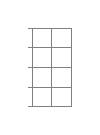
\begin{tikzpicture}[scale=0.5]
\draw[step=0.5,help lines] (1.9,0) grid (3,2);
\end{tikzpicture}
\end{tikzshow}

局部的缩放\latexline{clip}\tikzidx{clip}实现了剪裁的效果:
\begin{tikzshow}
\clip (-1.1,-1.1) rectangle (1.1,1.1);
\draw[step=1] (-2,-2) grid (2,1);
\end{tikzshow}

\tikzoptstyle{clip}与\tikzoptstyle{draw}实质都是\latexline{path}命令的参数的简写形式。使用该命令可以在剪裁时画出剪裁边缘:
\begin{tikzshow}
\path[clip,draw] (0,-0.5) circle [radius=1.2];
\draw[step=1] (-2,-2) grid (2,1);
\end{tikzshow}

剪裁命令在剪裁后经常需要放大,配合\tikzoptstyle{scale}选项较多。

\subsection{自定义}
选项\tikzoptstyle{help lines}实质是\tikzoptstyle{style=very thin, gray}的联合。使用\latexline{tikzset}\tikzidx{tikzset}命令设置它:
\begin{tikzshow}
\tikzset{help lines/.style = {color=blue,very thin}}
\draw[step=0.5,help lines] (0,0) grid (2,2);
\end{tikzshow}

或者在使用环境时直接将其作为选项写上:
\begin{tikzshow}
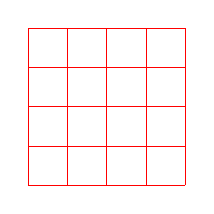
\begin{tikzpicture}[help lines/.style = {color=red,very thin}]
\draw[step=0.5,help lines] (0,0) grid (2,2);
\end{tikzpicture}
\end{tikzshow}

你也可以自定义选项,并且带参数:
\begin{tikzshow}
\tikzset{mystyle/.style={very thick,color=#1!50},
mystyle/.default=blue}
\draw[mystyle] (0,2) -- (3,2);
\draw[mystyle=green!50!black] (0,0) -- (3,0);
\end{tikzshow}

\section{几何形状}
\subsection{圆与椭圆}
圆与椭圆有专门的选项\tikzopt{circle}与\tikzopt{ellipse},指定圆心和半径:
\begin{tikzshow}
\draw (1,1) circle (0.5);
\draw (1,1) ellipse (1 and 0.5);
\end{tikzshow}

也可以写全参数:
\begin{tikzshow}
\draw (0,0) circle [radius=10pt];
\draw (0,0) ellipse [x radius=20pt, y radius=10pt];
\end{tikzshow}

\subsection{圆弧与椭圆弧}
圆弧可以通过指定起点角度、终点角度、圆弧半径来绘制,选项\tikzopt{arc}:
\begin{tikzshow}
\draw (3,0) arc (0:30:3);
ndraw (-2,1) arc (180:-45:2 and 1)
%等价:\draw (3,0) arc [start angle=0,end angle=30,radius=3];
\end{tikzshow}

类似地绘制椭圆弧:
\begin{tikzshow}
\draw (0,0) arc (0:270:0.7 and 0.4);
\end{tikzshow}

\subsection{矩形}
矩形的命令是\tikzopt{rectangle},指定左下角点和右上角点:
\begin{tikzshow}
\draw (0,0) rectangle (2,1);
\end{tikzshow}

\subsection{圆角与倒角}
选项\tikzopt{rounded corners}和\tikzopt{sharp corners}控制圆角和倒角。默认值是4\texttt{pt}。
\begin{tikzshow}
\draw [rounded corners] (0,0) -- (1,1)
-- (2,0) .. controls (3,1) .. (4,0);
\end{tikzshow}

如果写在两个点之间,可以“开关”圆角和尖角:
\begin{tikzshow}
\draw (0,0) [rounded corners=10pt] -- (1,1) -- (2,1)
[sharp corners] -- (2,0)
[rounded corners=5pt] -- cycle;
\end{tikzshow}

\subsection{抛物线*}
并不常用的\tikzopt{parabola}以及\tikzopt{bend},请读者自行理解:
\begin{tikzshow}
\draw (0,0) rectangle (1,1.5) (0,0) parabola (1,1.5);
\draw[xshift=1.5cm] (0,0) rectangle (1,1.5) (0,0) parabola[bend at end] (1,1.5);
\draw[xshift=3cm] (0,0) rectangle (1,1.5) (0,0) parabola bend (.75,1.75) (1,1.5);
\draw[yshift=-2cm] (1,1.5) --(0,0) parabola cycle;
\end{tikzshow}

其中\tikzoptstyle{bend}的含义是“拐点”,平常理解即一阶导数符号变化的点。理解:
\begin{tikzshow}
\draw[color=blue] (0,0) parabola[bend pos=0.25] (3,3);
\draw (0,1) parabola[parabola height=2cm] (3,0);
\end{tikzshow}

\subsection{填充与渐变}
填充命令\latexline{fill}\tikzidx{fill}只能用于闭合对象,需要\tikzopt{cycle}选项或者手动闭合到第一个点。也可以在填充的同时绘制,使用\latexline{filldraw}\tikzidx{filldraw}命令\footnote{颜色命令可能需要\pkg{xcolor}宏包。}。
\begin{tikzshow}
\fill[green] (0,0)--(1,0)--(0,1)--cycle;
\filldraw[fill=blue!50!white,draw=black] (1,0)--(3,0) arc (0:30:2) -- cycle;
\end{tikzshow}

填充还能根据重叠次数来判断填充与否,\tikzopt[fill]{even odd rule}例子:
\begin{tikzshow}
\fill[even odd rule, blue] (0,0) -- (2,0.5) -- (1,1) circle (0.25);
\end{tikzshow}

类似的渐变命令是\latexline{shade}\tikzidx{shade}和\latexline{shadedraw}\tikzidx{shadedraw}:
\begin{tikzshow}
\shade (0,0) rectangle (0.5,4);
\shade[top color=green,bottom color=white] (1,0) rectangle (1.5,2.5);
\shadedraw[left color=blue,right color=white] (1,3) rectangle (3,4);
\shade[inner color=yellow,outer color=black] (1.8,1.5) rectangle (3,2.5);
\shade[ball color=cyan] (2.4,0.75) circle (0.5);
\end{tikzshow}

上例的\tikzopt[shade]{ball}只是一种渐变类型,默认是\tikzopt[shade]{axis},另外还有\tikzopt[shade]{radial}可选。在\tikzoptstyle{axis}下,还可以选择渐变角度\tikzoptstyle{shading angle}。
\begin{tikzshow}
\shade[shading=radial,inner color=orange] (0,0) rectangle (3,1.5);
\shade[shading angle=45,right color=lime] (0,1.5) rectangle (3,3);
\end{tikzshow}

\section{坐标系与坐标}
\subsection{箭头}
绘制坐标系的方法非常基础,使用带箭头的直线:
\begin{tikzshow}
\draw[->] (1,2)--(2,2); 
\draw[<-] (1,1)--(2,1); % 反过来画
\draw[<->] (0,2.5)--(0,0)--(2.5,0);
\draw[|<->|] (1.5,0.5)--(1.5,2.5); % 很实用
\end{tikzshow}

也有一些其他风格的箭头,更多的请调用\pkg{arrows.meta}这个库。
\begin{tikzshow}
\draw[-latex] (0,3)--(2,3);
\draw[-stealth] (0,2.5)--(2,2.5);
\draw[-to] (0,2)--(2,2);
\draw[-to reversed] (0,1.5)--(2,1.5);
\end{tikzshow}

\subsection{极坐标与相对坐标}
直角坐标的表示非常简单,比如(0,1)。也可以指定单位,比如(0,1pt)。而极坐标则可以用(30:1)的方式表示在30$^\circ$方向上的1单位长位置的点。

加号可以用来指代相对坐标,是相对该语句中最后一个绝对坐标而言的;而两个加号用于移动“笔”的位置,是相对该语句最后一个坐标而言的。体会:
\begin{tikzshow}
\filldraw[fill=green!20,draw=green!50!black] (0,0) -- (0.5,0)
arc [start angle=0, end angle=30, radius=0.5] -- cycle;
\draw[red,very thick] (30:2) -- +(0,-1);
\draw[blue,very thick] (30:2) ++(0,-1) -- (0,0);
\end{tikzshow}

\subsection{横纵坐标投影}
这个命令是象形的:\tikzoptstyle{-|}与\tikzoptstyle{|-}两种。
\begin{tikzshow}
\draw (0,0)--(2,1) -| cycle;
\draw (1.5,0)--(3,1) |- cycle;
\end{tikzshow}

\section{输出单个文件}
要输出为\texttt{.svg}矢量文件,用于更多的插图场合。需要在电脑安装pdf2svg\footnote{\url{http://www.cityinthesky.co.uk/opensource/pdf2svg/}}。不过在\LaTeX 使用的场合,可以去掉下述的\texttt{convert}参数,以输出\texttt{.pdf}格式的矢量文件。

下例中的\texttt{multi=false}表示只输出为单页文件。

\begin{latex}
\documentclass[tikz,convert=pdf2svg,multi=false]{standalone}
% tikz package already loaded by 'tikz' option
\begin{document}
\begin{tikzpicture}
  \draw (0,0) -- (10,10);
  \draw (10,0) -- (0,10);
\end{tikzpicture}
\end{document}
\end{latex}

在编译时如果是\xelatex ,还需要添加参数:
\begin{latex}
% 如果上例的文件名为 example.tex
xelatex -shell-escape example.tex
\end{latex}

\endinput


% 参考文献
\begin{thebibliography}{9}

\bibitem{mittelbach2004latex} Goossens, Michel, Frank Mittelbach, and Alexander Samarin.
  \newblock \emph{The \LaTeX\ Companion}, 2nd edition.
  \newblock Addison-Wesley Reading Mass, 2004.

\bibitem{partl2016} Hubert Partl, Irene Hyna, and Elisabeth Schlegl.
  \newblock \emph{一份不太简短的\LaTeX 2$\varepsilon$介绍}.
  \newblock China\TeX 论坛译, 2016. \\
  English: \url{https://www.ctan.org/tex-archive/info/lshort/english}\\
  中文: \url{https://github.com/CTeX-org/lshort-cn/releases}
  
\bibitem{Casteleyn2016tikz} Jean Pierre Casteleyn.
  \newblock \emph{Visual TikZ (version 0.62)}.
  \newblock IUT Génie Thermique et Énergie, 2016. \\
  \url{http://tug.ctan.org/info/visualtikz/VisualTikZ.pdf}
      
\bibitem{lamport1986document} Leslie Lamport.
  \newblock \emph{\LaTeX: A Document Preparation System}, 2nd edition.
  \newblock Addison-Wesley Reading Mass, 1994.
  
\bibitem{LHY2013latex} 刘海洋.
  \newblock \emph{\LaTeX 入门}.
  \newblock 电子工业出版社, 2013.

\end{thebibliography}

\endinput


\clearpage
\begin{appendices}
%\renewcommand{\CTEXthechapter}{\Alph{chapter}}
\titleformat{\chapter}[display]{\Huge\bfseries}{附录\Alph{chapter}}{1em}{}

\chapter{注音符号}
\label{app:phonetic}
% 这里不用>{\ttfamily}而用\verb是为了减少报错可能
\begin{center}
\tabcaption{注音符号与特殊符号}
\begin{tabular}{|*{4}{>{\centering}p{3em} @{-\hspace{1em}} p{3em}|}}
\hline
\texttt{样式} & 命令 & \texttt{样式} & 命令 & \texttt{样式} & 命令 & \texttt{样式} & 命令 \\
\hline
\=o  & \verb|\=o|  & \'o  & \verb|\'o|  & \v o & \verb|\v o|  & \`o   & \verb|\`o|  \\
\^o  & \verb|\^o|  & \"o  & \verb|\"o|  & \.o  & \verb|\.o|   & \H o  & \verb|\H o| \\
\d o & \verb|\d o| & \u o & \verb|\u o| & \b o & \verb|\b o|  & \t oo & \verb|\t oo|\\
\multicolumn{2}{|c@{\bf --}}{$\tilde{o}$} & \multicolumn{2}{@{\bf --}c|}{\tt{\$$\backslash$tilde\{o\}\$}} &%
\multicolumn{2}{c@{\bf --}}{$\hat{o}$}    & \multicolumn{2}{@{\bf --}c|}{\tt{\$$\backslash$hat\{o\}\$}}\\
\multicolumn{8}{|c|}{} \\
\o  & \verb|\o|  & \O  & \verb|\O|  & \i  & \verb|\i|  & \j  & \verb|\j| \\
\aa & \verb|\aa| & \AA & \verb|\AA| & \ae & \verb|\ae| & \AE & \verb|\AE|\\
\oe & \verb|\oe| & \OE & \verb|\OE| & !`  & \verb|!`|  & ?`  & \verb|?`| \\
\hline
\end{tabular}
\end{center}

\mbox{}

\begin{center}
\tabcaption{国际音标输入表(部分)}
\begin{tabular}{|*{3}{>{\rmfamily}c !{-} >{\ttfamily}p{7.5em}|}}
\hline
\texttt{样式} & 命令 & \texttt{样式} & 命令 & \texttt{样式} & 命令 \\
\hline
\textdzlig & \char92textdzlig & \textesh & \char92textesh & \textteshlig & \char92textteshlig \\
\textdyoghlig & \char92textdyoghlig & \textturnv & \char92textturnv & \textschwa & \char92textschwa \\
\textscriptg & \char92textscriptg & \texttheta & \char92texttheta & \textupsilon & \char92textupsilon \\
\textscripta & \char92textscripta & \dh & \char92dh & \textepsilon & \char92textepsilon \\
\textopeno & \char92textopeno & \textyogh & \char92textyogh & \ng & \char92ng \\
\hline
\multicolumn{2}{|c|}{重音} & \multicolumn{2}{c|}{次重音} & \multicolumn{2}{c|}{长音节} \\
\textprimstress & \char92{}textprimstress & \textsecstress & \char92textsecstress & \textlengthmark & \char92textlengthmark \\
\hline
\end{tabular}
\end{center}

\textit{注:\texttt{\char92dh}命令在非CJK文档中有时编译会出现问题}。

\chapter{建议}
除了参考文献列表中给出的书籍以外,我还推荐你用控制台在\TeX{} Live中能找到的以下书籍:

\begin{para}
\item[texdoc usrguide] \TeX Live自带的用户手册。
\item[texdoc clsguide] \TeX Live自带的文档类和宏包学习手册。
\item[texdoc fntguide] \TeX Live自带的字体使用手册。
\item[texdoc symbols-a4] 一份速查表,基本上所有的\LaTeX 字符命令都在这里了。
\item[texdoc latexcheat] 很有趣的命令表,只有两页。
\item[texdoc impatient] \textit{\TeX{} for the Impatient}, 一本介绍底层\TeX 的书,中译本资源请自己寻找。这也是我阅读的第一本\TeX 书,Knuth的\textit{The \TeX book}虽然血统正但是难啃啊。
\item[texdoc texbytopic] \textit{\TeX{} by Topic}, 个人觉得不如上面那本,但也许只是叙述方式不一样吧。
\end{para}

\end{appendices}

\end{document}
